\subsection{Designing Guess that Number} % (fold)
\label{sub:designing_guess_that_number}

Table \ref{tbl:control-flow-prog} contains a description of the next program we are going to design. This program plays a small guessing game called \emph{Guess that Number}. In this game the computer will think of a target number between 1 and 100. The user then has 7 guesses to determine the target number's value. At each guess the computer outputs a message to indicate if the target number is greater than, less than, or equal to the user's guess.

\begin{table}[h]
\centering
\begin{tabular}{l|p{10cm}}
  \hline
  \multicolumn{2}{c}{\textbf{Program Description}} \\
  \hline
  \textbf{Name} & \emph{Guess that Number} \\
  \\
  \textbf{Description} & A simple guessing game where the computer `thinks' of a number between 1 and 100, and the user has seven guesses to guess it. With each guess the computer indicates if the number it is thinking of is less than, or greater than the user's guess. If the user runs out of guesses they are shown the answer, and that round ends. After each round the user has the option to play again, or to quit the program.\\
  \hline
\end{tabular}
\caption{Description of the Guess That Number program.}
\label{tbl:control-flow-prog}
\end{table}

As before, the process to design and implement this program will follow a number of steps:
\begin{enumerate}
  \item Understand the problem, and get some ideas on the tasks that need to be performed.
  \item Choose the artefacts we will create and use
  \item Design the control flow for the procedural\footnote{The program, and any Functions and Procedures.} artefacts
  \item Map these artefacts to code
  \item Compile and run the program
\end{enumerate}

The new step in this process will involve designing the flow of the instructions within the program, and the Functions and Procedures that need to be created. Previously each artefact had a sequential flow of instructions, the introduction of the control flow statements has made it possible to add branches and loops to this sequence. The order of these actions needs to be considered for each sequence of instructions in your code.

% subsection designing_guess_that_number (end)

\clearpage
\subsection{Understanding Guess that Number} % (fold)
\label{sub:understanding_guess_that_number}

Guess that Number is a relatively common game involving one player choosing a number, and the other trying to guess it. Each guess is followed by an indication of whether the guess was less than or larger than the target number. The game continues until the player guesses the target number.

The data for this program will be relatively simple. The code will need to keep track of the current \textbf{target number} which will be an integer. The player will be able to enter a \textbf{guess}, also an integer. These two numbers represent the data model for the game. It is a game that involves a \emph{target number} and \emph{guess}.

The actions within the program involve \textbf{playing the game}, and \textbf{performing a guess}. Playing the game is the process of performing guesses until the player finally guesses the target number. This version of the game will only allow the player to have seven guesses, so this will need to be a part of this code in the program. The process of performing a guess will involve getting the user's guess, and giving them feedback indicating if they guessed the target number, of if they were larger than, or less than the target.

% subsubsection understanding_guess_that_number (end)

\subsection{Choosing Artefacts for Guess that Number} % (fold)
\label{sub:choosing_artefacts_for_guess_that_number}

Software design is all about \textbf{abstraction}. This is the process of determining the essential features of the problem and modelling that in the artefacts that you create in your code. When designing the artefacts that will make up your code you need to think about problem, and try to create artefacts in your code that represent the actions and data you imagine when thinking about the problem.

Our understanding of the Guess that Number game indicates that there are two processes that need to be performed within the program: \textbf{play game} and \textbf{perform guess}. These two processes can be coded as either Functions or Procedures in the Program's code. The \texttt{Play Game} code can be implemented as a \nameref{sub:procedure}. It will be responsible for running the process of the game, starting with telling the user it has `thought of a number', through to coordinating the guesses, ending only when the user gets the answer of runs out of guesses.

\texttt{Perform Guess}, on the other hand, will need to be a \nameref{sub:function} as it must return back a \nameref{sub:boolean_data} value indicating if the user has guessed the number. The code in \texttt{Perform Guess} will be responsible for asking the user to enter a guess, and then giving them the feedback on their guess. As this has the details of the guess, its result is needed to allow \texttt{Play Game} to determine if the user has guessed the number.

The \texttt{Perform Guess} code will also need to accept parameters to tell it what the current \texttt{target} value is. This data will exist within the \texttt{Play Game} code, so it will need a mechanism to pass that code to \texttt{Perform Guess}. A \nameref{sub:parameter} is needed in \texttt{Perform Guess} to accept \texttt{target} will enable this. 

A nicety may be to allow tell the user which guess they are up to. Once again, this information is stored in \texttt{Play Game}, so a second parameter can be added to allow \texttt{Play Game} to pass in the \texttt{guess number} along with the \texttt{target} number.

In addition to these it has been decided to add a \texttt{Print Line} procedure to display a line of `-' characters. This will be displayed at the end of the game before the user is asked if they want to play again. A \texttt{length} parameter will enable the caller to indicate how many of these characters are printed on the line.

The Structure Chart showing these artefacts is shown in Figure \ref{fig:guess-game-structure}, and the Sequence Diagram is shown in Figure \ref{fig:guess-game-seq}. Notice that there is some relationship here between the artefacts that we are creating and the steps in the game itself. The earlier it is to see the relationship between these artefacts and the problem, the better job you have done abstracting your solution.

\begin{figure}[htbp]
   \centering
   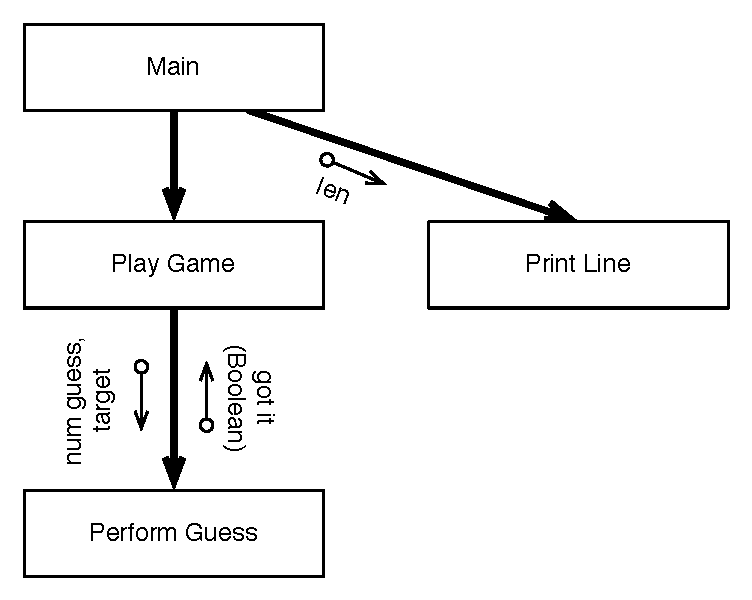
\includegraphics[width=0.6\textwidth]{./topics/control-flow/diagrams/GuessThatNumStructure} 
   \caption{Structure Chart for the Guess that Number Program}
   \label{fig:guess-game-structure}
\end{figure}

\begin{figure}[htbp]
   \centering
   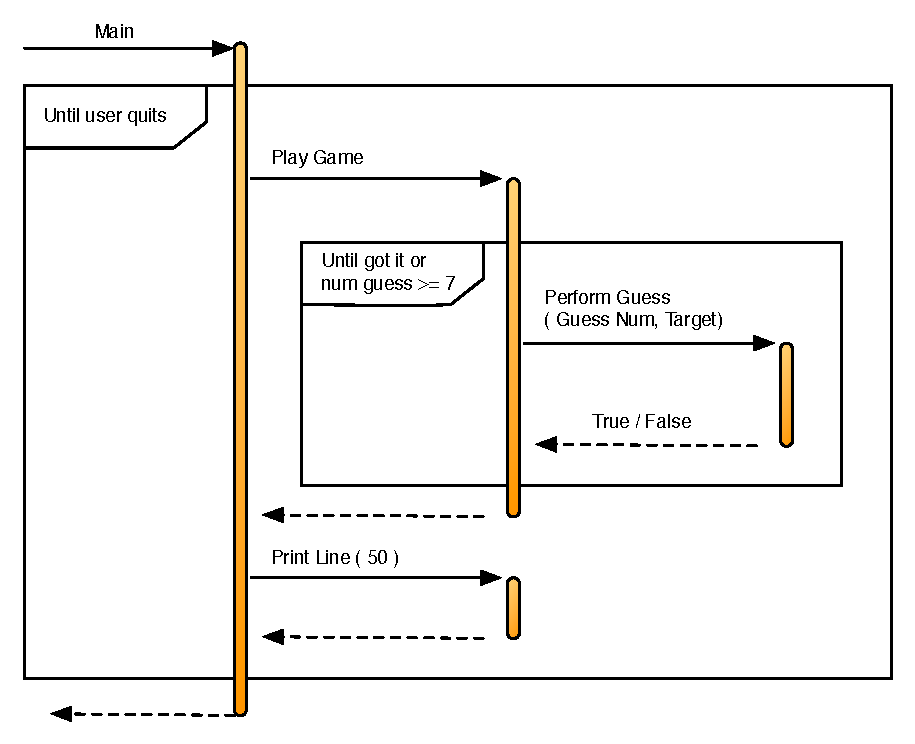
\includegraphics[width=\textwidth]{./topics/control-flow/diagrams/GuessThatNumSeq} 
   \caption{Sequence Diagram for the Guess that Number Program}
   \label{fig:guess-game-seq}
\end{figure}
% subsection choosing_artefacts_for_guess_that_number (end)

\clearpage
\subsection{Designing Control Flow for Perform Guess} % (fold)
\label{sub:designing_control_flow_for_perform_guess}

Having chosen the artefacts to build, the next step is to design the control flow that will enable these Functions and Procedures, and the program itself, to achieve their goals. Each has a responsibility that it must meet in order for the overall solution to work. 

This section will go through designing the logic for the \texttt{Perform Guess} Function. It will cover the following points: 
\begin{itemize}
  \item \nameref{ssub:flow_charts}
  \item \nameref{ssub:structured_programming}
  \item \nameref{ssub:structured_programming_blocks}
  \item \nameref{ssub:combining_blocks_for_the_guessing_game}
  \item \nameref{ssub:setting_the_result_using_an_expression}
  \item \nameref{ssub:the_pseudocode_for_perform_guess}
\end{itemize}

\subsubsection{Drawing control flow using a Flowchart} % (fold)
\label{ssub:flow_charts}

Before examining the control flows within the Functions and Procedures of the Guess that Number program, let us have a look at a means of visually representing flow of actions within code. A common means of doing this is to use a \textbf{flowchart}. This is a diagram that depicts a sequence of actions, and can be used to represent the sequence of action actions that occur within your code.

The flowchart has four basic symbols as shown in Figure \ref{fig:flow-symbols}.
\begin{itemize}
  \item \textbf{Start/Stop}: This represents the start and end of the process. Typically the start node would have the name of the Function or Procedure within it.
  \item \textbf{Flow}: The arrows between nodes represent control flow, indicating which action is to be performed next in the code.
  \item \textbf{Process}: This node represents a task being performed. In our case this will map to one, or more, simple statements. The text in the Process node should indicate what is being performed at this stage.
  \item \textbf{Decision}: This represents a point where the code needs to make a decision. This is used for the conditions in the \nameref{sub:branching} and \nameref{sub:looping} statements. A decision \textbf{must} have more than one flow coming out of it, and each flow should indicate the condition that triggers that path.
\end{itemize}

\begin{figure}[htbp]
   \centering
   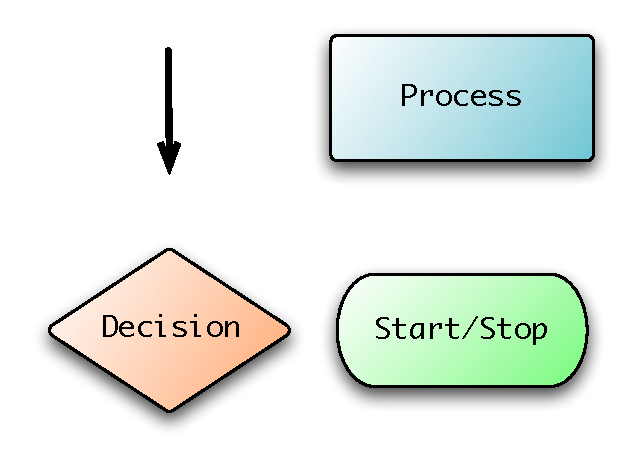
\includegraphics[width=0.5\textwidth]{./topics/control-flow/diagrams/FlowParts} 
   \caption{Flowchart Symbols}
   \label{fig:flow-symbols}
\end{figure}

% subsubsection flow_charts (end)

\clearpage
\subsubsection{Use Structured Programming Principles to guide the design of the flowchart} % (fold)
\label{ssub:structured_programming}

Flowcharts can be used to represent any sequence of actions, but not all sequences of actions will be easy to code. \fref{fig:unstructured-flow-example} is an example of a flowchart, but not one that can be coded using the structured statements covered in \cref{cha:control_flow}. \fref{fig:structured-flow-example} shows a structured version of this same algorithm. Notice that in this version there are identifiable blocks, each having a single entry and a single exit. This structure could easily be converted to code using structured statements. 

Looking at these two flowcharts, the structured flowchart looks more complicated than the unstructured version. This reflects the fact that in some cases the structured version may be more complicated, but is also an indication that this process may be better broken down into more functions and procedures. For example, the repeated loop looking for someone else to blame could be placed in its own procedure. If you find it difficult to design the control flow using structured blocks try to see if you can identify additional Functions and Procedures to help you break the code down into smaller blocks. 

\begin{figure}[htbp]
   \centering
   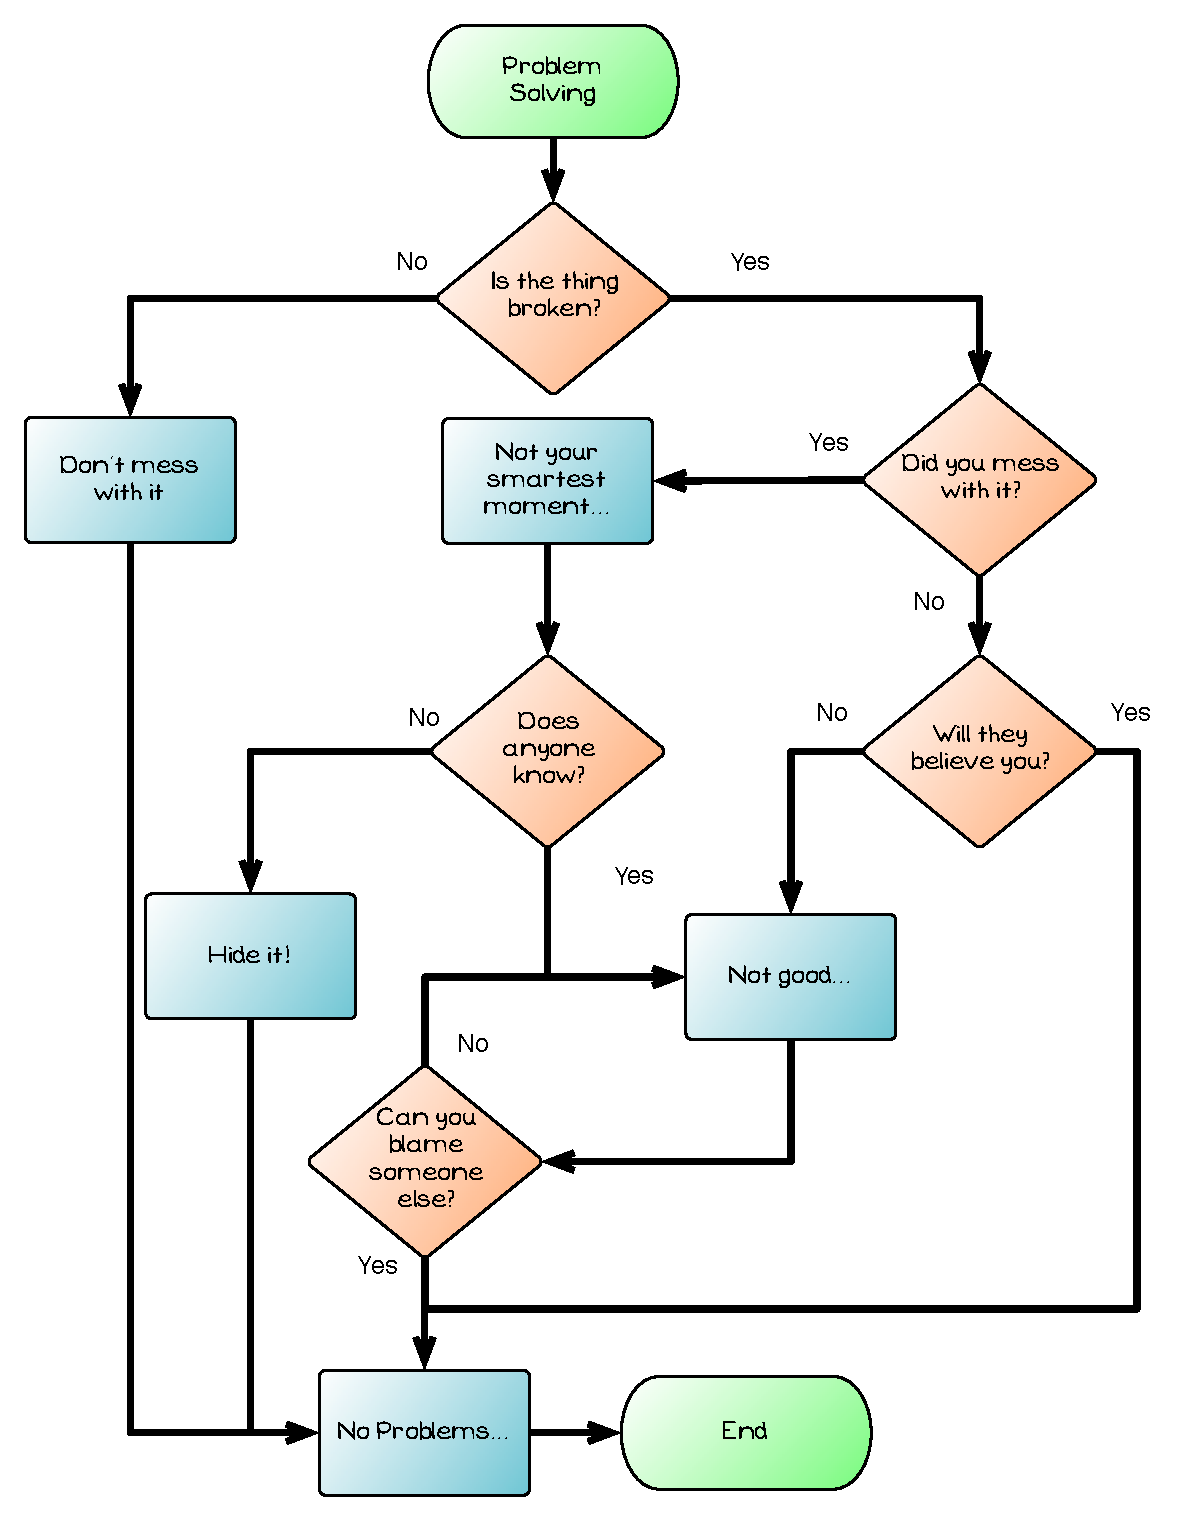
\includegraphics[width=\textwidth]{./topics/control-flow/diagrams/UnstructuredFlowSample} 
   \caption{Unstructured Flowchart}
   \label{fig:unstructured-flow-example}
\end{figure}

\begin{figure}[htbp]
   \centering
   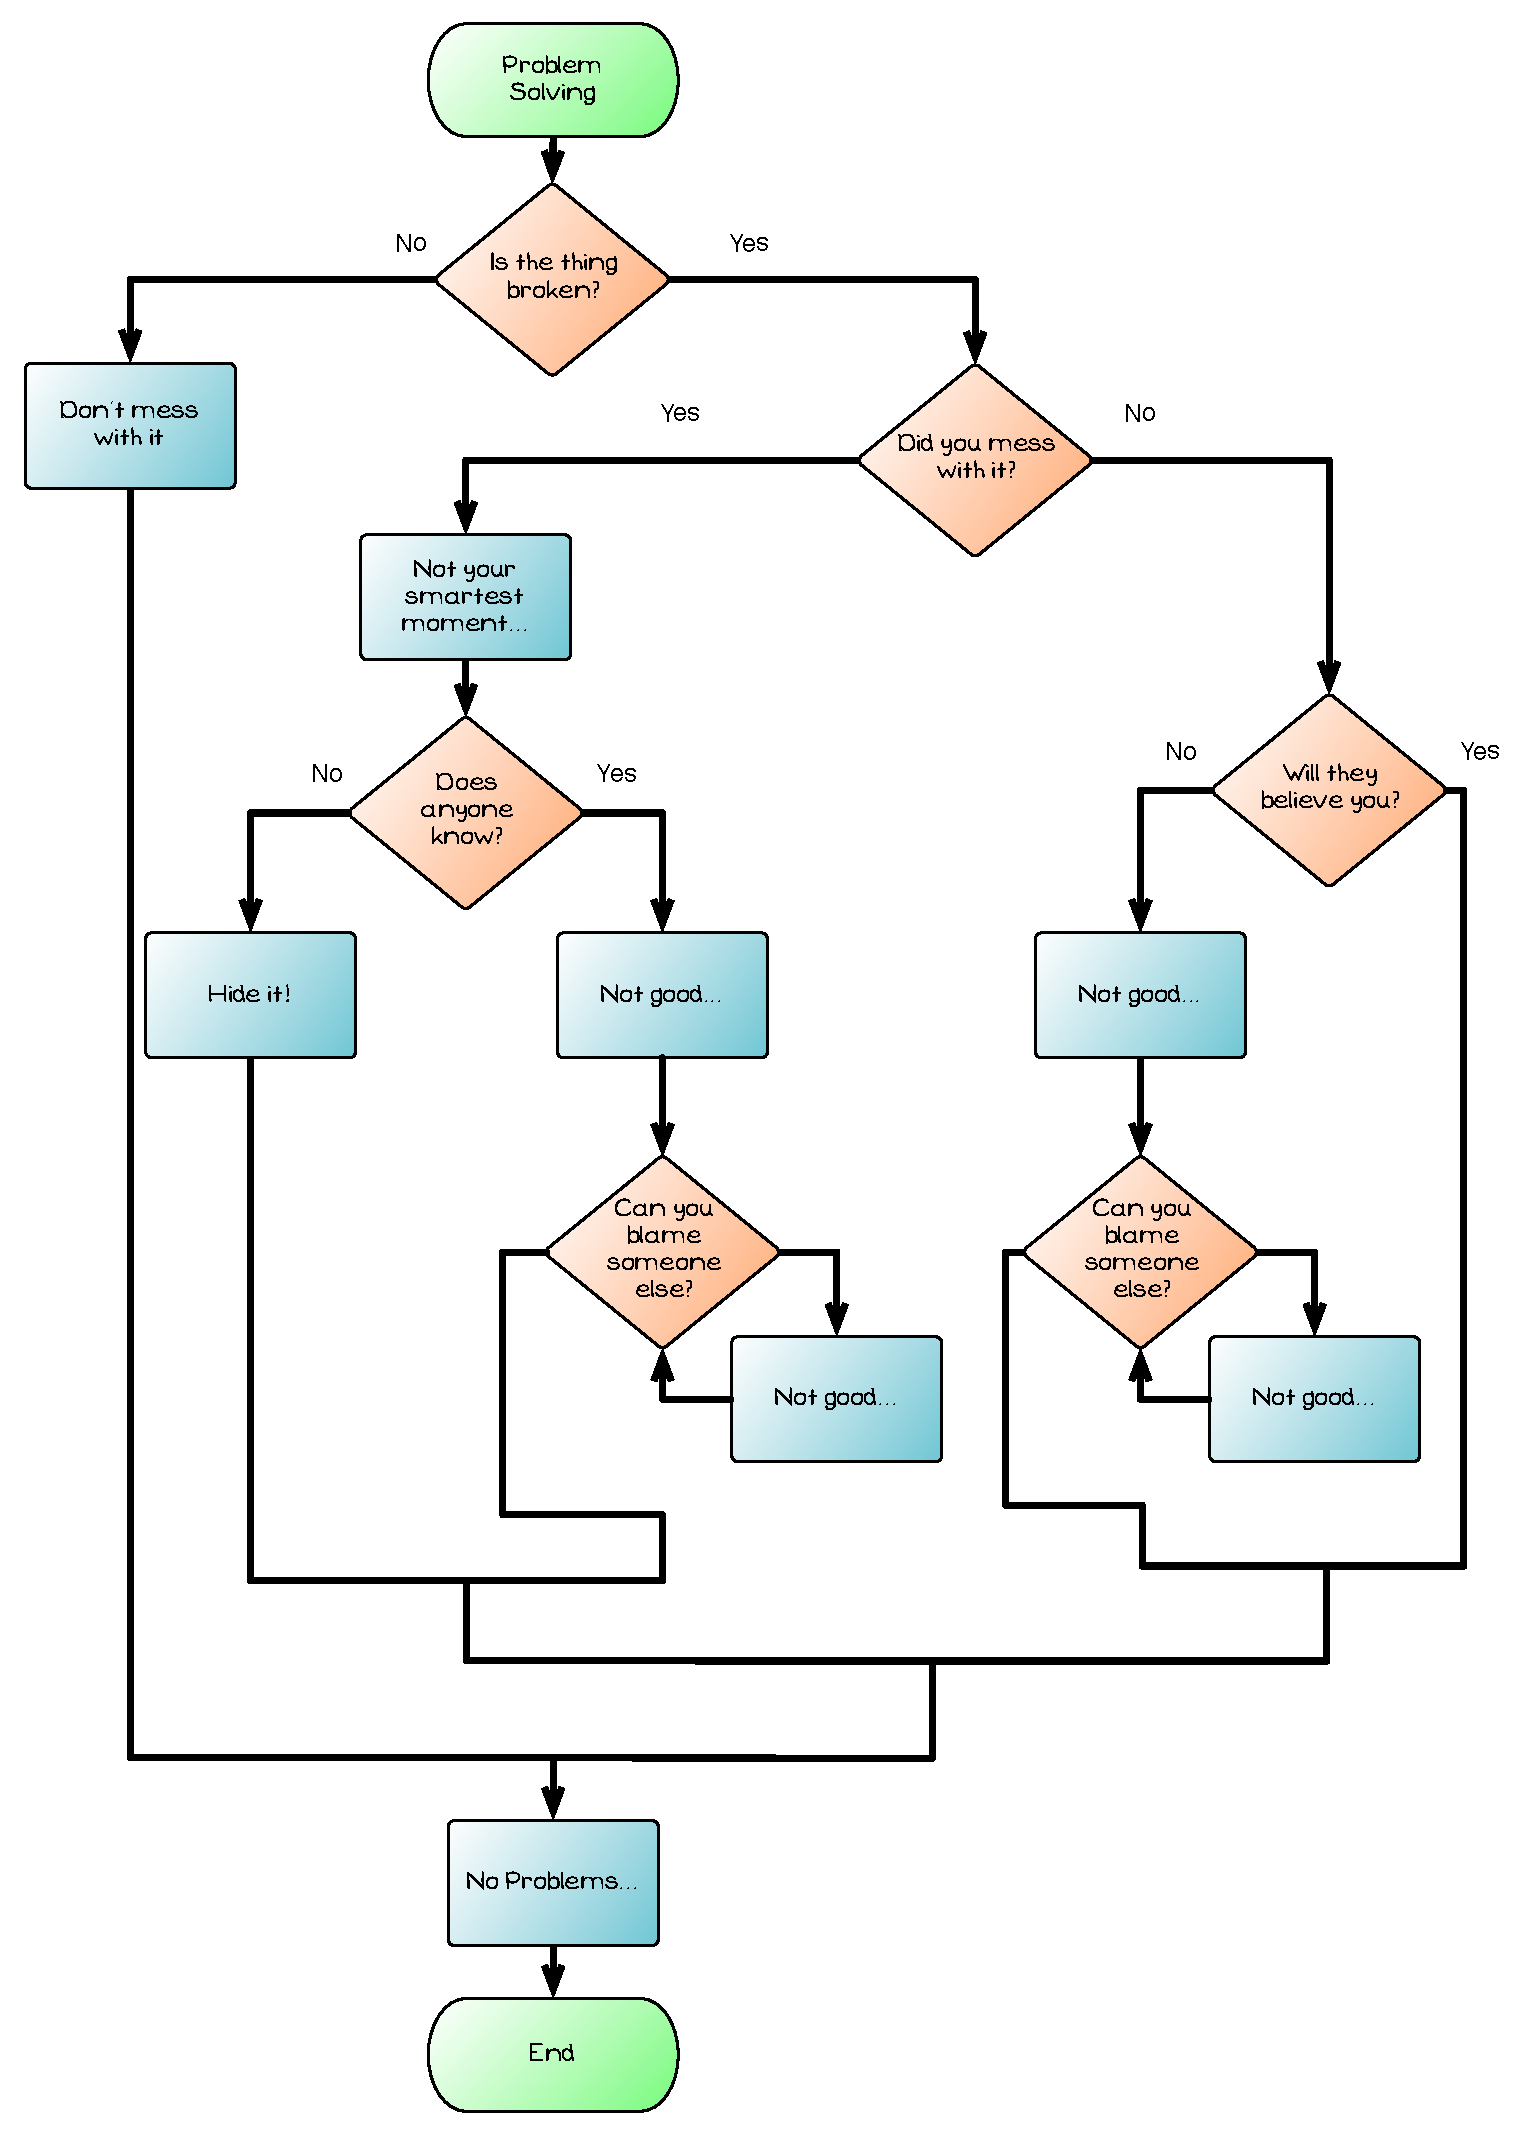
\includegraphics[width=\textwidth]{./topics/control-flow/diagrams/StructuredFlowSample} 
   \caption{Structured version of Figure \ref{fig:unstructured-flow-example}}
   \label{fig:structured-flow-example}
\end{figure}

The structured programming principles indicate that code within a Function or Procedure should be organised into \textbf{blocks}. These blocks match to the structured statements in modern programming languages: the \nameref{sub:branching} and \nameref{sub:looping} statements. Each of these blocks has a \textbf{single entry point} and a \textbf{single exit point}, allowing them to combined together.

The addition of \nameref{sub:jump} statements to the language allows the blocks to have \textbf{multiple exit points}; one at the end of the block's code, the other at a \nameref{sub:break}, \nameref{sub:exit}, or \nameref{sub:return_statement}. These statements give you extra flexibility, but still work within the structured programming principles.

\mynote{
Prior to the Structured Programming, programs had two control flow mechanisms: \texttt{if} and \nameref{sub:goto}. Control flow was not easy to picture or understand. Programs written in this way are now know as \textbf{spaghetti code}, as understanding this code is much like trying to untangle a bowl of spaghetti, though not nearly as tasty.
}
% subsubsection structured_programming (end)

\clearpage
\subsubsection{The Structured Programming blocks used to build the logic} % (fold)
\label{ssub:structured_programming_blocks}

In Structured Programming there are three kinds of blocks:
\begin{itemize}
  \item \textbf{Sequence}: one instruction follows the next in a sequence.
  \item \textbf{Selection}: the ability to branch the sequence.
  \item \textbf{Repetition}: repeat a block a number of times.
\end{itemize}

The flowchart snippets in the section on \nameref{sub:branching} and \nameref{sub:looping} showed how the flows work for \emph{selection} and \emph{repetition}. \fref{fig:selection-flow} shows the three alternatives for selection blocks, \fref{fig:repetition-flow} shows the two alternatives for repetition blocks, and \fref{fig:sequence-flow} shows the standard sequence flow. The design of any program's logic is a task in combining these blocks together to perform the desired effect. 

\begin{figure}[h]
   \centering
   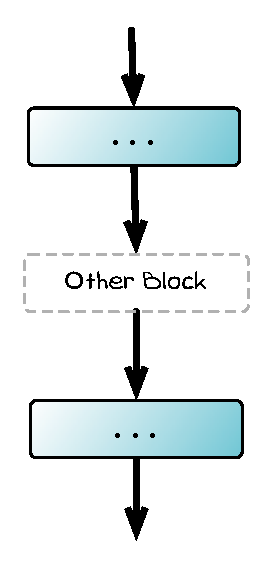
\includegraphics[width=0.15\textwidth]{./topics/control-flow/diagrams/SequenceFlow} 
   \caption{Flows for Sequence Blocks}
   \label{fig:sequence-flow}
\end{figure}

\begin{figure}[h]
   \centering
   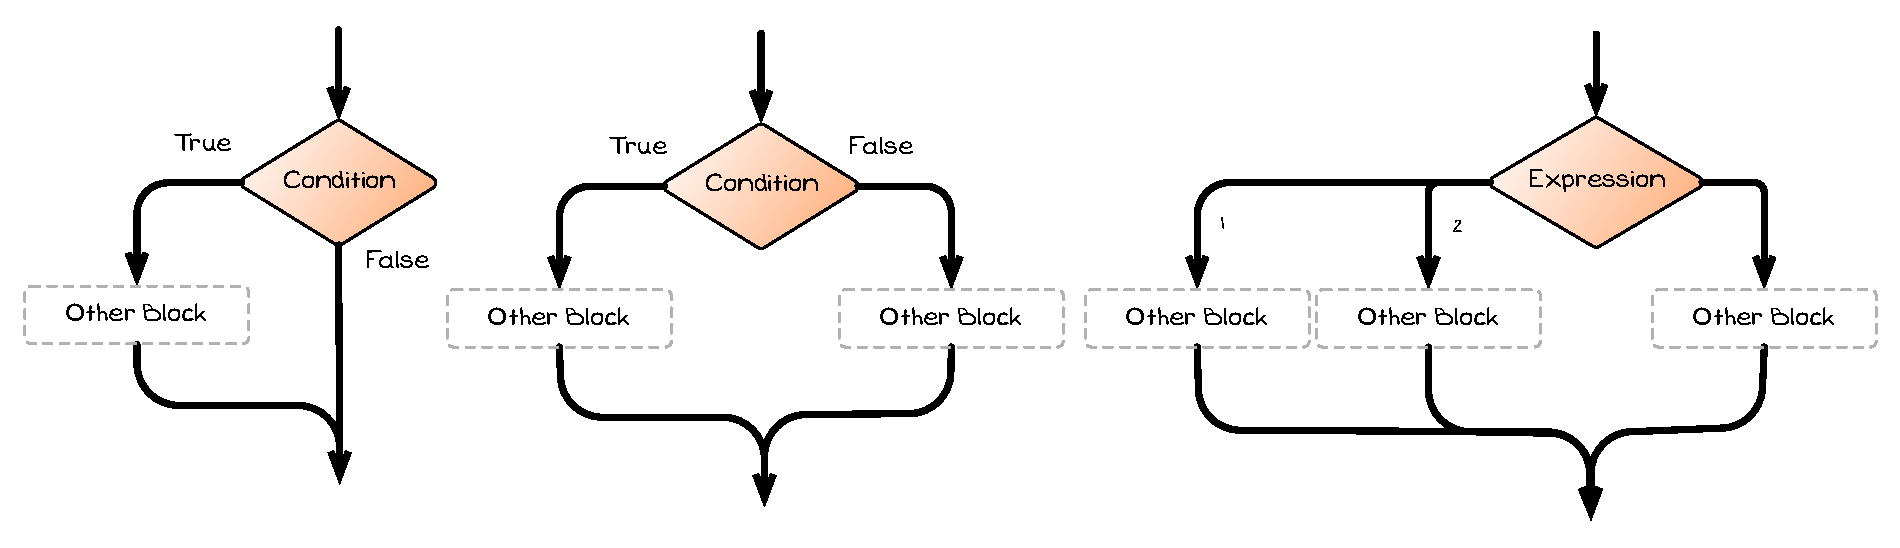
\includegraphics[width=0.9\textwidth]{./topics/control-flow/diagrams/SelectionFlow} 
   \caption{Flows for Selection Blocks}
   \label{fig:selection-flow}
\end{figure}

\begin{figure}[h]
   \centering
   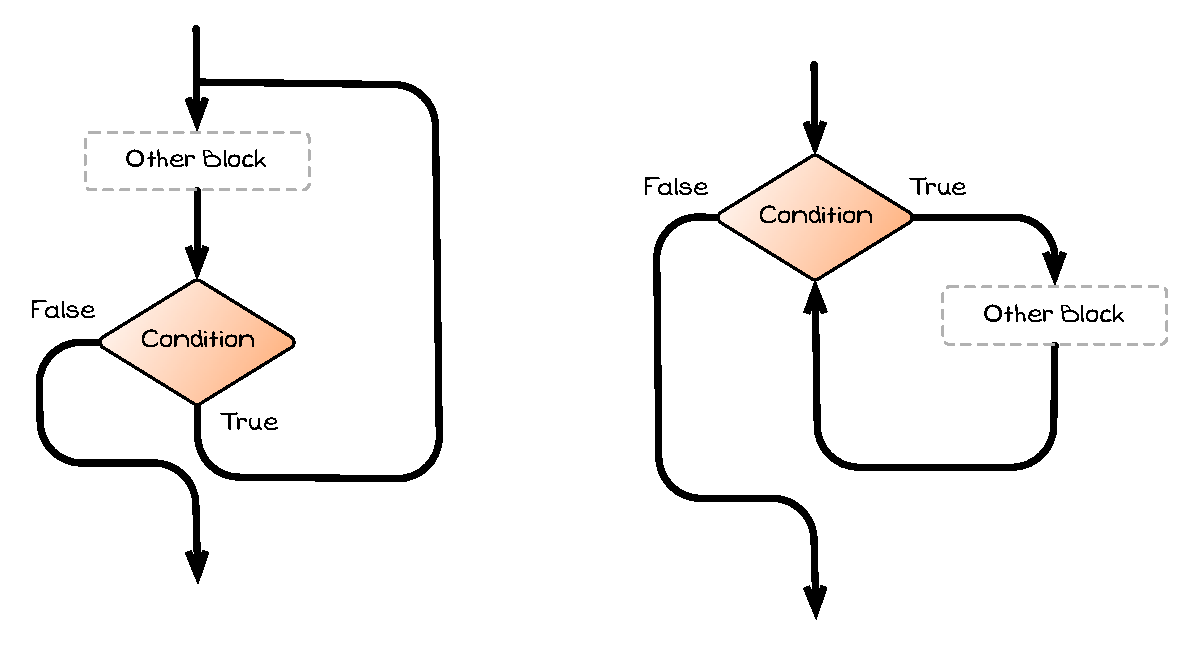
\includegraphics[width=0.55\textwidth]{./topics/control-flow/diagrams/RepetitionFlow} 
   \caption{Flows for Repetition Blocks}
   \label{fig:repetition-flow}
\end{figure}

% subsubsection structured_programming_blocks (end)

\subsubsection{Combining blocks for the Perform Guess} % (fold)
\label{ssub:combining_blocks_for_the_guessing_game}

With the basic theory at hand, we can now start to design the control flow for the Guess that Number program. This process will involve, once again, the idea of \textbf{abstraction}. When designing the flow for a program you first need to be able to perform the process yourself, even if its just on paper, and then work out the steps that you undertook so that you can code these within the program.

For the Guess that Number program we can start by designing the control flow within the \texttt{Perform Guess} function. The specification of this is shown in \tref{tbl:perform guess}. Think about the steps that need to be performed to achieve this. If you had been asked to do this what would you need to do?

\begin{table}[h]
  \centering
  \begin{tabular}{|c|p{9cm}|}
    \hline
    \multicolumn{2}{|c|}{\textbf{Function}} \\
    \hline
    \multicolumn{2}{|c|}{} \\
    \multicolumn{2}{|c|}{\texttt{Perform Guess}} \\
    \multicolumn{2}{|c|}{} \\
    \hline
    \multicolumn{2}{|c|}{\textbf{Returns}} \\
    \hline
    \texttt{Boolean} & True when the user has guessed the number, False otherwise. \\
    \hline
    \textbf{Parameter} & \textbf{Description} \\
    \hline
    \texttt{Guess Number} & The number of the current guess, used in the prompt asking for the user to enter their guess. \\
    & \\
    \texttt{Target}   & The number the user is aiming to guess. \\
    \hline
    \multicolumn{2}{|c|}{} \\
    \multicolumn{2}{|p{12cm}|}{Perform Guess is responsible for coordinating the actions needed to perform a single guess within a game of \emph{Guess that Number}. The user's \texttt{guess} is read, and the value checked against the \texttt{target} value. A message is then output telling the user if the target value is less than, larger than, or equal to their guess. This function returns True when the user's guess is equal to the target.} \\
    \multicolumn{2}{|c|}{} \\
    \hline
  \end{tabular}
  \caption{Specification for the \texttt{Perform Guess} Function.}
  \label{tbl:perform guess}
\end{table}

The first task the Function needs to perform is to get the guess from the user. This can be performed in a \textbf{sequence}: display a prompt, read the value from the user. This first sequence is shown in \fref{fig:perform-guess-seq-1}.

\begin{figure}[h]
   \centering
   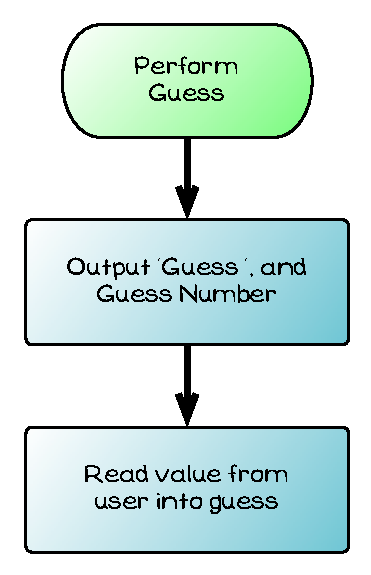
\includegraphics[width=0.25\textwidth]{./topics/control-flow/diagrams/PerformGuess1} 
   \caption{Initial Sequence in \texttt{Perform Guess}}
   \label{fig:perform-guess-seq-1}
\end{figure}

\clearpage
The next step in this sequence is to give the user feedback based upon their guess and the target number. This code requires a the ability to \emph{select} a given branch. The computer needs to output different messages based upon the users guess. This can be achieved with a \textbf{selection} block. Looking back at \fref{fig:selection-flow} there are three possible alternatives for implementing this selection. The \texttt{if} with no \texttt{else} is not a valid option as there are three paths we need to take. The \texttt{case} block is also not valid as we are not matching a value, but comparing values to each other. The last option is the \texttt{if-else} block, but this only has two branches. It is not going to be possible to code all three options within one block, but it can be achieved using two \texttt{if-else} blocks.

The first \texttt{if-else} block will check if the \texttt{target} is greater than the user's \texttt{guess}. If this is true then the computer can take the first branch and output the message `The number is larger than ' and the value from the user's guess. The flow chart for this part is shown in \fref{fig:perform-guess-seq-2}. This block is the third task in the sequence, this if block has a single entry, causes a branch in the flow, and will have a single exit.

\begin{figure}[h]
   \centering
   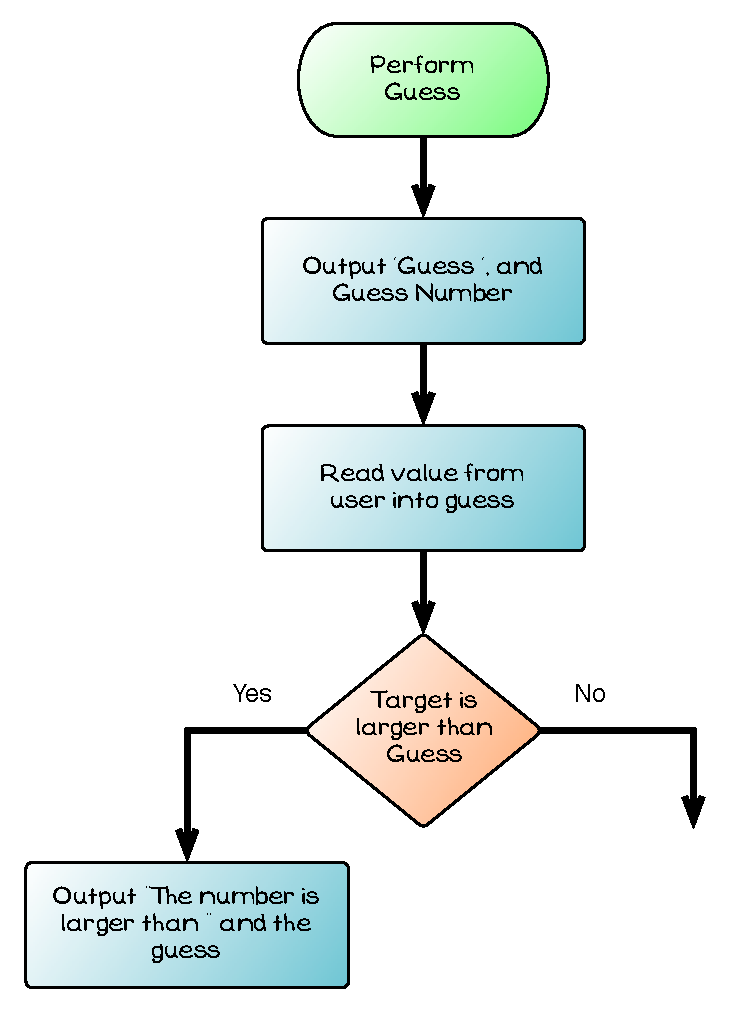
\includegraphics[width=0.6\textwidth]{./topics/control-flow/diagrams/PerformGuess2} 
   \caption{First branch in \texttt{Perform Guess}}
   \label{fig:perform-guess-seq-2}
\end{figure}

\mynote{
\begin{itemize}
  \item The conditions within the \nameref{sub:if_statement} are Boolean Expressions.
  \item This condition is checking if \texttt{target > guess}.
  \item There are now two paths through this code, one when \texttt{target} is \texttt{> guess}, and another when it is not.
\end{itemize}
}

\clearpage

Following the false path from the first decision, and we have a new location into which to insert a block. At this point we know the target is \emph{not} larger than the user's guess. At this point you can include another \texttt{if-else} block to check if the target is \textbf{less than} the user's guess. This is shown in \fref{fig:perform-guess-seq-3}.

\begin{figure}[htbp]
   \centering
   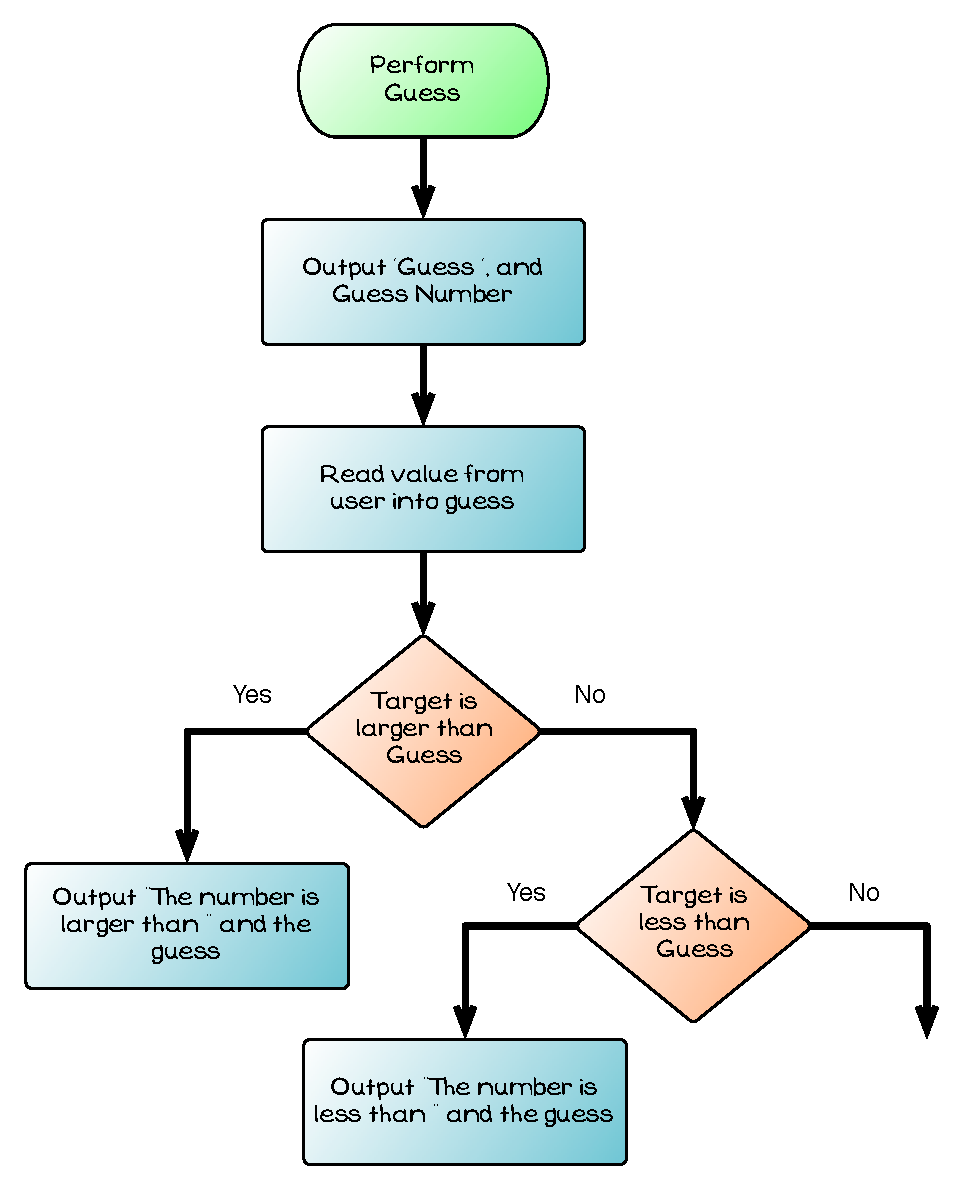
\includegraphics[width=0.7\textwidth]{./topics/control-flow/diagrams/PerformGuess3} 
   \caption{Second branch tests if the Target is less than the guess}
   \label{fig:perform-guess-seq-3}
\end{figure}

\mynote{
\begin{itemize}
  \item The newly added block is another \nameref{sub:if_statement}.
  \item This is nested within the \texttt{else} branch of the first If Statement.
  \item This code checks \emph{if} \texttt{target < guess}.
  \item There are now three paths through this code.
\end{itemize}
}

\clearpage
Taking the false path again, and now we have a location at which the target value \emph{must be} equal to the user's guess. The first condition checked if the \texttt{target} was larger than the \texttt{guess}, which it was not. The second condition checked if the \texttt{target} was less than the \texttt{guess}, which it was not. So the only way this can be the case if is the \texttt{target} and the \texttt{guess} are equal. This path can then be used to output the `Well done\ldots' message. This is shown in \fref{fig:perform-guess-seq-4}. 

\begin{figure}[htbp]
   \centering
   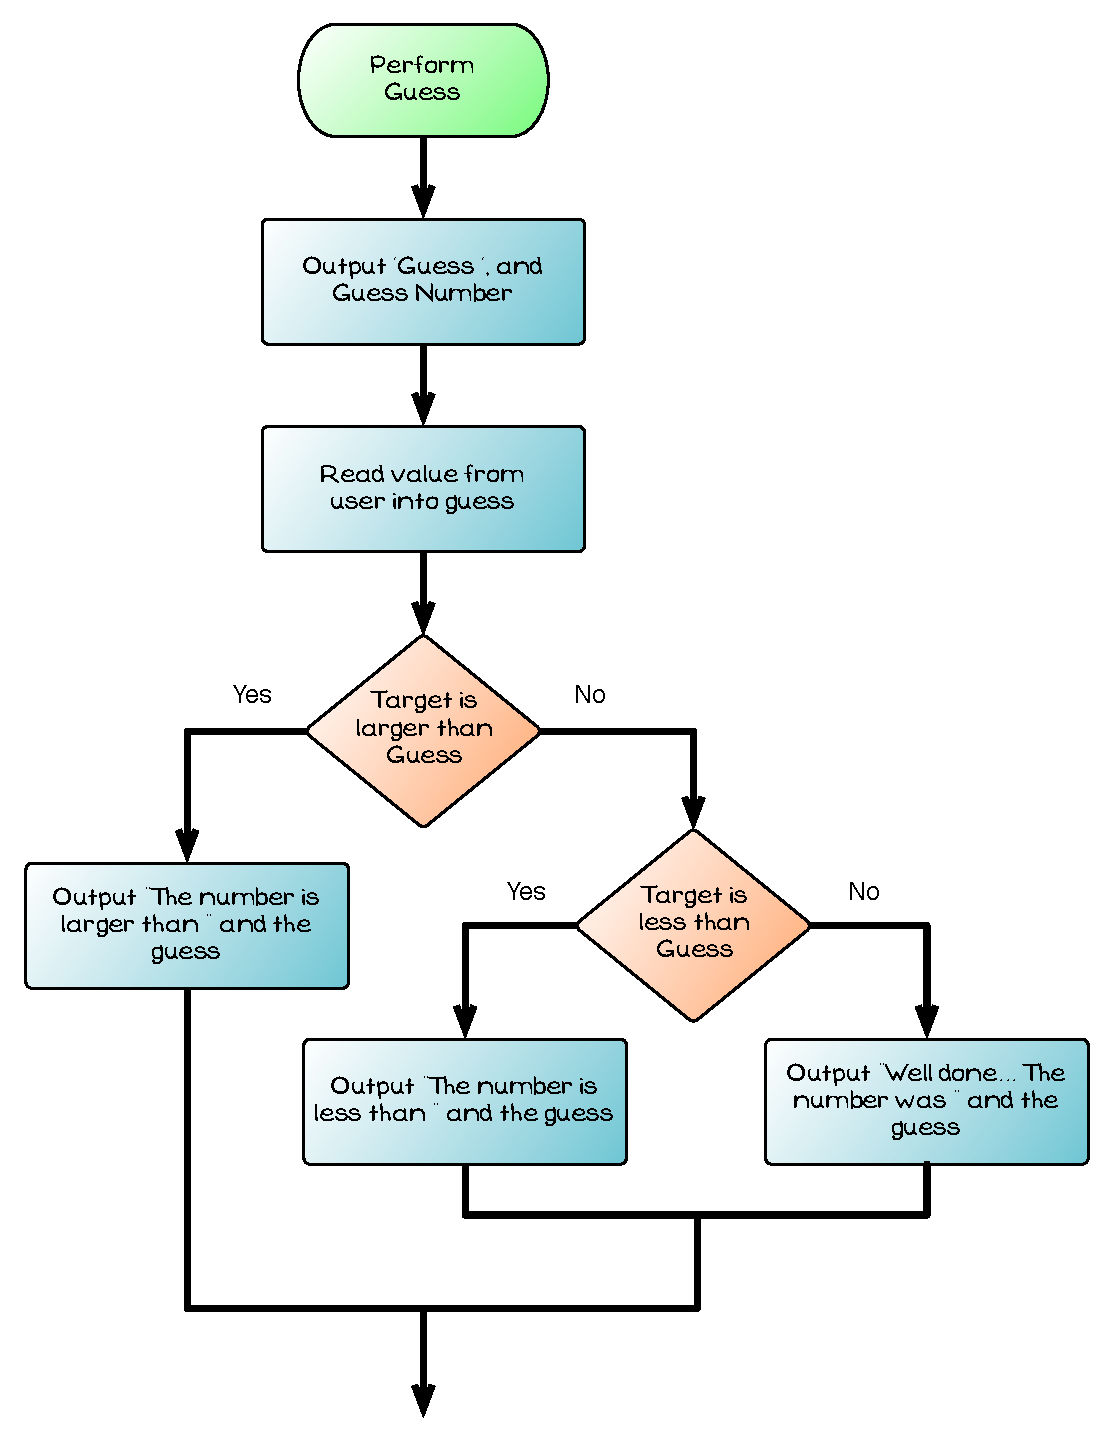
\includegraphics[width=0.8\textwidth]{./topics/control-flow/diagrams/PerformGuess4} 
   \caption{The `Well done\ldots' message can be output on the third path}
   \label{fig:perform-guess-seq-4}
\end{figure}

\mynote{
\begin{itemize}
  \item The newly added block is a sequence, outputting the `Well done\ldots' message.
  \item On this third path the \texttt{target} and \texttt{guess} must be equal.
  \item Notice the single exit out of the second branch, when then flows to the single exit out of the first branch.
\end{itemize}
}

\clearpage
The last action in the code is to return a Boolean result indicating if the user's guess is equal to the target number.

\begin{figure}[htbp]
   \centering
   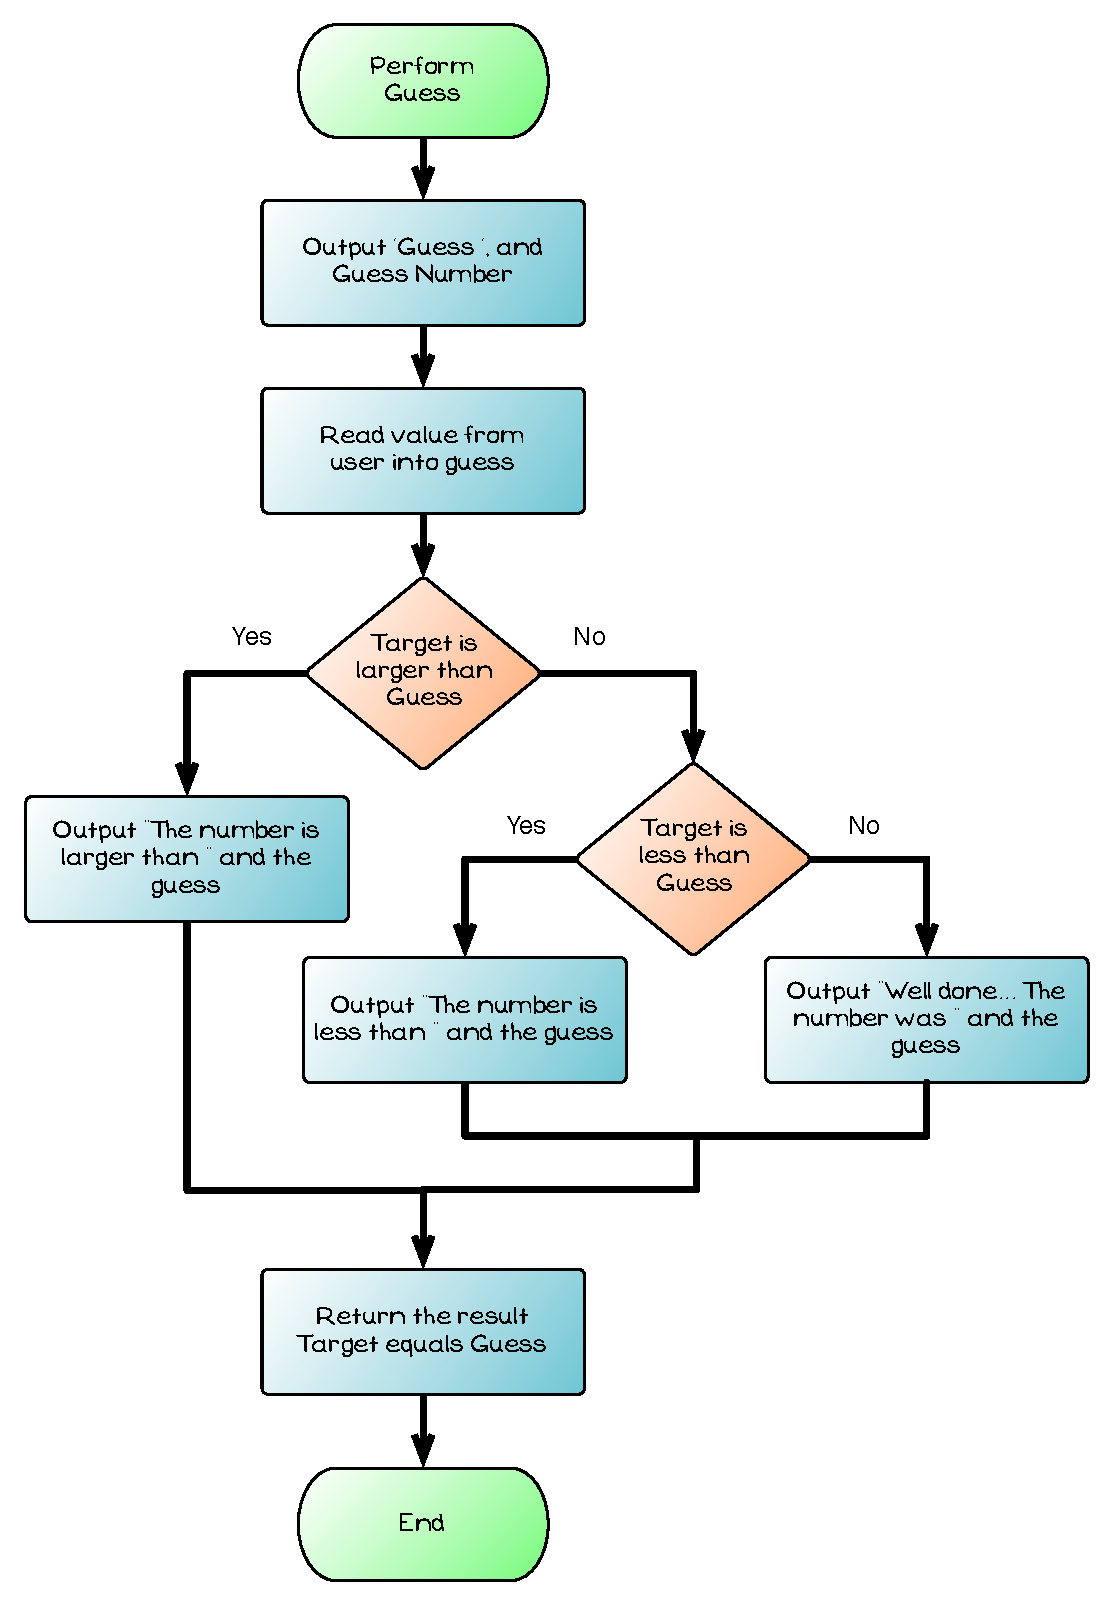
\includegraphics[width=0.74\textwidth]{./topics/control-flow/diagrams/PerformGuess5} 
   \caption{A Boolean result is returned from the Function}
   \label{fig:perform-guess-seq-5}
\end{figure}

\mynote{
\begin{itemize}
  \item The newly added block is a single action, defining the result to be returned.
  \item This action returns the result True when the \texttt{target} and the \texttt{guess} are equal.
\end{itemize}
}

\clearpage

\fref{fig:perform-guess-seq-7} shows the flowchart with annotations highlighting the different blocks within the code. The function starts off with a \textbf{sequence} that contains all of the code in the Function. Within this there is the \textbf{selection}, that internally contains another \textbf{selection}.

\begin{figure}[htbp]
   \centering
   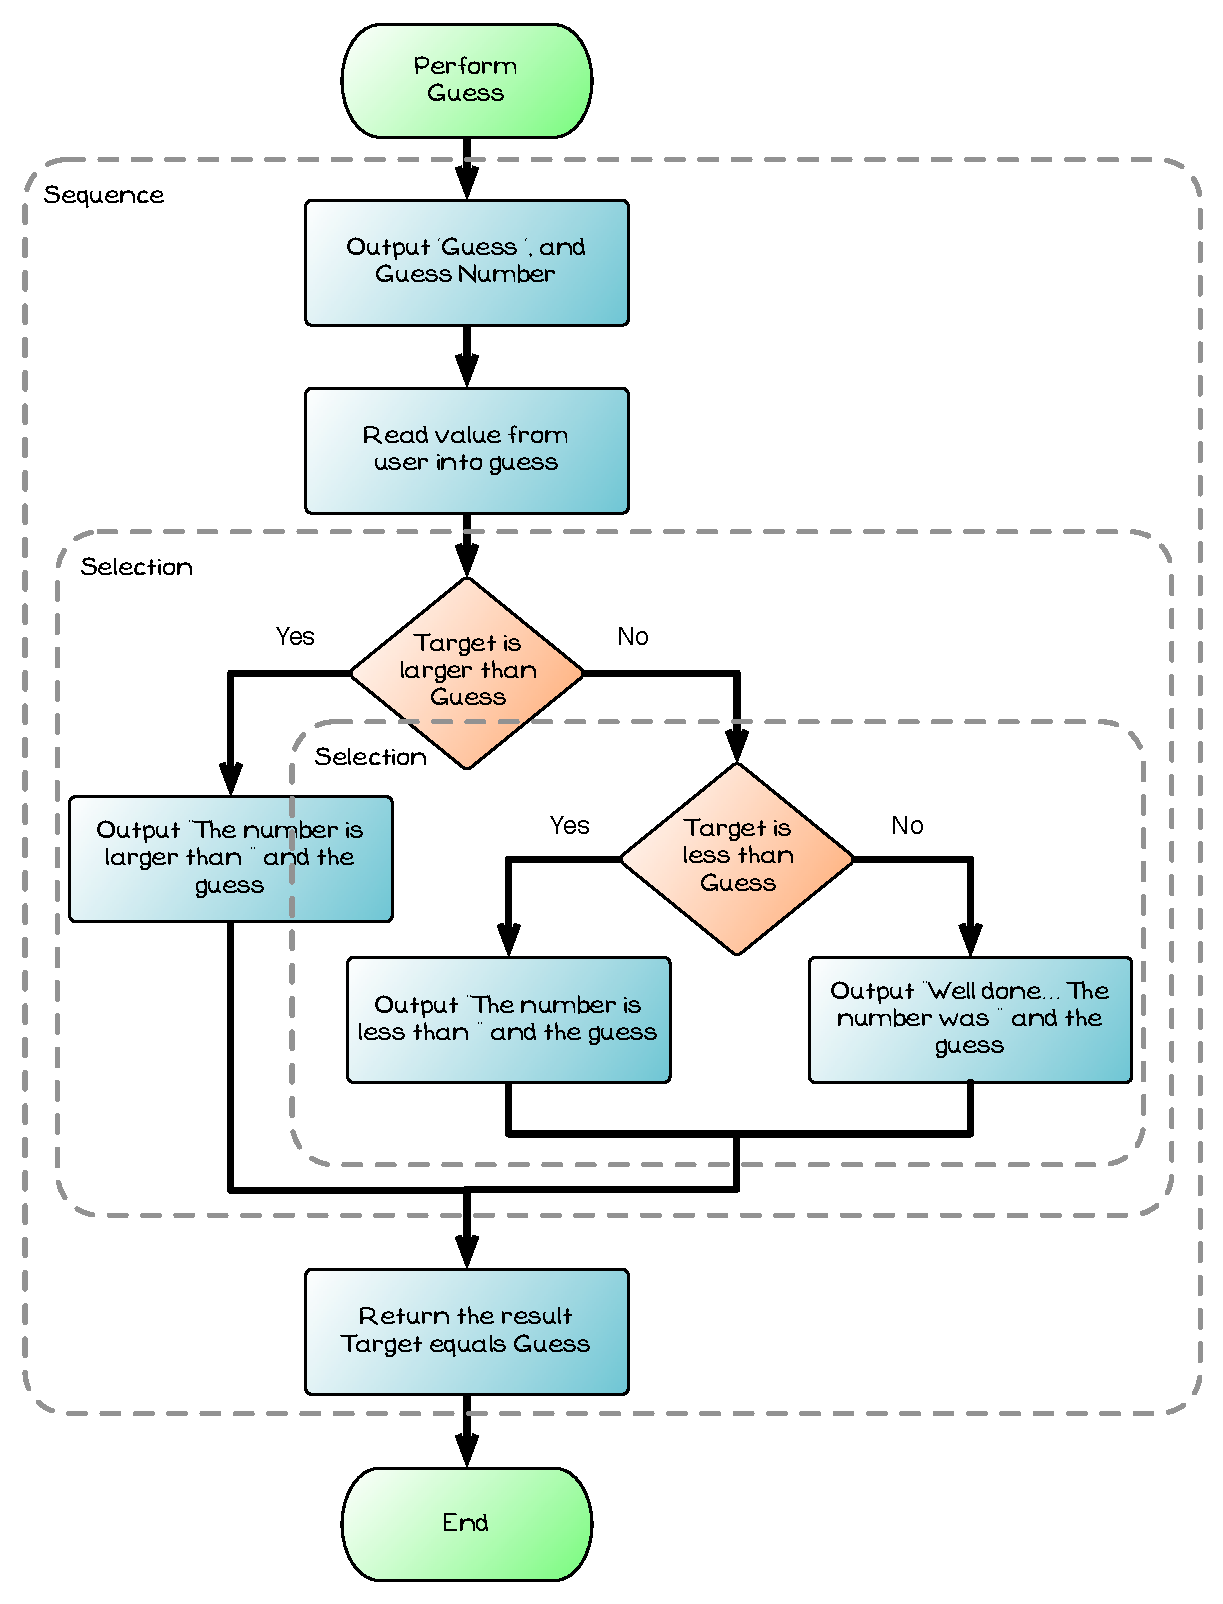
\includegraphics[width=0.85\textwidth]{./topics/control-flow/diagrams/PerformGuess7} 
   \caption{Blocks in the \texttt{Perform Guess} code}
   \label{fig:perform-guess-seq-7}
\end{figure}

\mynote{
\begin{itemize}
  \item Notice that each block has a single path going into it, and a single path coming out.
\end{itemize}
}

% subsubsection combining_blocks_for_the_guessing_game (end)

\clearpage
\subsubsection{Setting the result using an Expression} % (fold)
\label{ssub:setting_the_result_using_an_expression}

\fref{fig:perform-guess-seq-6} shows the \emph{trick} that is being performed at the end of \texttt{Perform Guess}'s code. \texttt{Perform Guess} needs to return a result indicating if the user has guessed the number of not. This will be a Boolean value, with True indicating they guessed the number. Initially it may seem that you need a \textbf{selection} block to enable this, as shown on the right of \fref{fig:perform-guess-seq-6}. 

\begin{figure}[htbp]
   \centering
   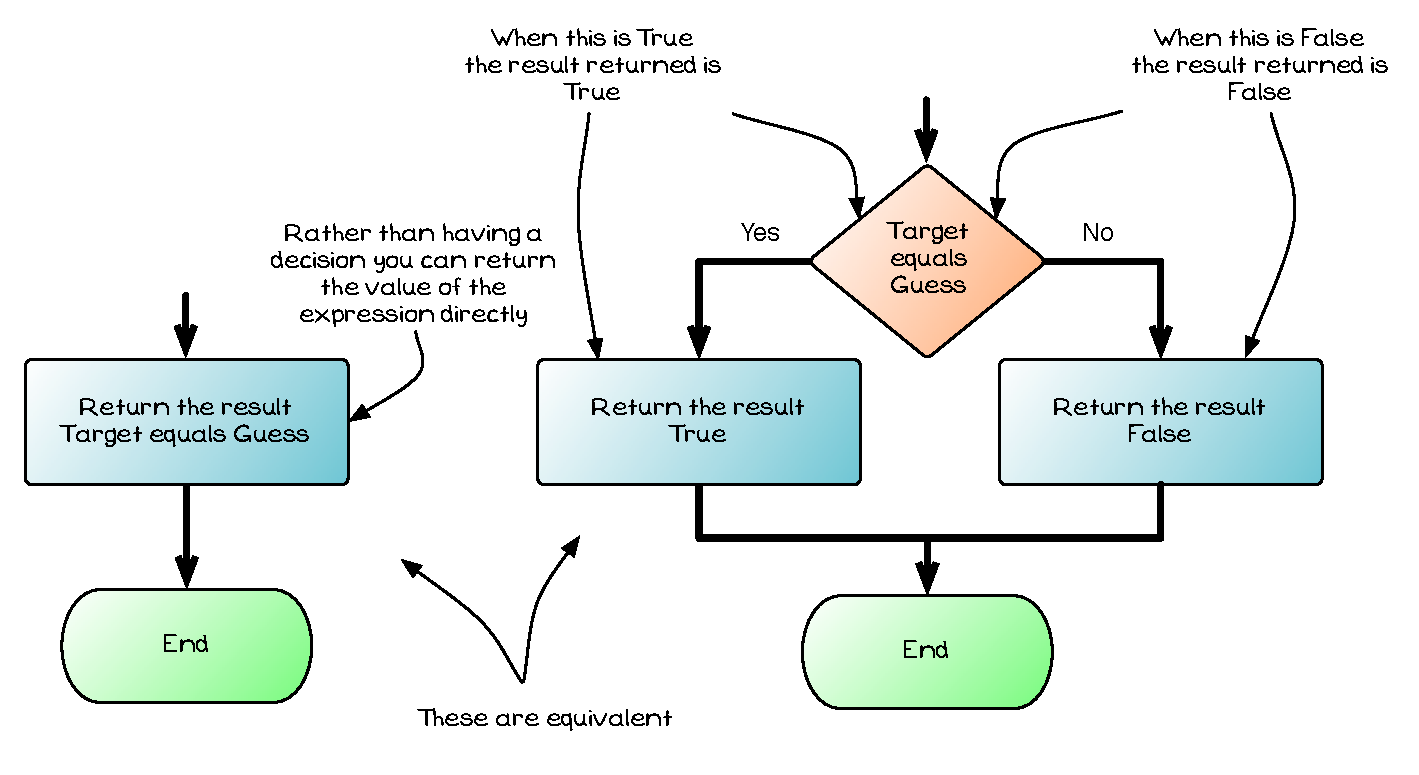
\includegraphics[width=\textwidth]{./topics/control-flow/diagrams/PerformGuess6} 
   \caption{Calculating \texttt{Perform Guess}'s result}
   \label{fig:perform-guess-seq-6}
\end{figure}

\mynote{
\begin{itemize}
  \item In \emph{most} cases it is better to have less code if possible, as long as this does not obscure the purpose of the code.
  \item This is an example of replacing \emph{actions} with \emph{data}. The more \emph{intelligence} you can build into the data in your programs the more flexible they will be.
\end{itemize}
}

\csection{This is achieved in C using \csnipet{return target == guess;}}

\passection{This is achieved in Pascal using \passnipet{result := target = guess;}}


% subsubsection setting_the_result_using_an_experssion (end)

\clearpage
\subsubsection{The Pseudocode for \texttt{Perform Guess}} % (fold)
\label{ssub:the_pseudocode_for_perform_guess}

Listing \ref{plst:perform_guess} contains the Pseudocode for the \texttt{Perform Guess} logic from the flowchart in \fref{fig:perform-guess-seq-5}. Notice how the indentation in this mirrors the block structures in the flowchart. It is good practice to indent your code in this way as it helps you, and any person who reads your code, to see the structure of the logic. You will be able to avoid many errors by making sure that you always indent your code so that it highlights the code's structure.

\pseudocode{plst:perform_guess}{Pseudocode for \texttt{Perform Guess}}{topics/control-flow/application/PerformGuess.txt}

\mynote{
\begin{itemize}
  \item Code indentation makes it easier to read, and helps locate many common issues.
  \item Tab you code in within a \textbf{structured statement}.
  \begin{itemize}
    \item Indent the code in the branches of an \nameref{sub:if_statement} and \nameref{sub:case_statement}.
    \item Indent the code within the body of the \textbf{While Loop} and the \textbf{Do While} or \textbf{Repeat Until} loops. 
  \end{itemize}
  \item Make this a habit. When you code a \nameref{sub:branching} or \nameref{sub:looping} statement automatically indent the next line of code.
  \item Always keep you code neat, make it look good.
  \item The C code for \texttt{Perform Guess} is shown in Listing \ref{clst:perform_guess}.
  \item The Pascal code for \texttt{Perform Guess} is shown in Listing \ref{paslst:perform_guess}.
  \item Notice how the two code samples are laid out in a similar way. The indentation makes it easy to identify which statements are associated with each of the branches through the Function. 
\end{itemize}
}

\clearpage

\csection{\ccode{clst:perform_guess}{C code for \texttt{Perform Guess}}{topics/control-flow/application/perform-guess.c}}

\passection{\pascode{paslst:perform_guess}{Pascal code for \texttt{Perform Guess}}{topics/control-flow/application/PerformGuess.pas}}


% subsubsection the_pseudocode_for_ (end)


% subsection designing_control_flow_for_guess_that_number (end)

\clearpage
\subsection{Designing Control Flow for Play Game} % (fold)
\label{sub:designing_control_flow_for_play_game}

The \texttt{Play Game} Procedure is another artefact that will require some some thought to design its logic. \tref{tbl:play game} contains the specification for this Procedure. It will be responsible for coordinating the actions of the game, while \texttt{Perform Guess} coordinates the actions for a \emph{single} guess.

\begin{table}[h]
  \centering
  \begin{tabular}{|c|p{9cm}|}
    \hline
    \multicolumn{2}{|c|}{\textbf{Procedure}} \\
    \hline
    \multicolumn{2}{|c|}{} \\
    \multicolumn{2}{|c|}{\texttt{Play Game}} \\
    \multicolumn{2}{|c|}{} \\
    \hline
    \multicolumn{2}{|c|}{} \\
    \multicolumn{2}{|p{12cm}|}{Play Game is responsible for coordinating the actions involved in playing a single game of \emph{Guess that Number}. Initially the computer will generate a random target value, and output starting text. Then it will repeatedly ask the user to guess the number, until either the user has guessed the value or they have run out of guesses. If the user does run out of guesses then the computer ends the game, and tell the user the target value.} \\
    \multicolumn{2}{|c|}{} \\
    \hline
  \end{tabular}
  \caption{Specification for the \texttt{Play Game} Procedure.}
  \label{tbl:play game}
\end{table}

The implementation of this Procedure will require us to store some data. The following \nameref{sub:local_variable}s will be needed to store data within this Procedure:
\begin{itemize}
  \item \texttt{\textbf{My Number}}: This will store the computer's randomly chosen number.
  \item \texttt{\textbf{Guess Number}}: This will store the current guess the user is at, allowing the computer to stop looping when the number of guesses is exceeds 7.
  \item \texttt{\textbf{Got It}}: A Boolean value to indicate if the user did guess the number, allowing the computer to stop looping when the user guesses the number.
\end{itemize}

The flowchart for this is shown in \fref{fig:play-game}, and again in \fref{fig:play-game-diag1} with its blocks highlighted. This code uses a \textbf{repetition} to ask the user to perform up to 7 guesses. The condition on this loop occurs \emph{after} the loop body as the user must have at least one guess. 

There is also a \textbf{selection} after the loop to output the answer if the user ran out of guesses. This is only done when the user has not guessed it themselves. This does not need to perform any other actions when the user did guess the number, so the False branch has no additional actions. In code this would be implemented with an \nameref{sub:if_statement} without an \textbf{else} branch.

\mynote{
\begin{itemize}
  \item A loop may have its condition before or after its instructions.
  \item If the condition is after the loop, as it is with \texttt{Play Game}, then this gives a loop that runs at least once.
  \item The else branch on the If Statement is optional. If you have no processing for this branch you leave the \texttt{else} off in the code.
  \item The condition of the If Statement in \texttt{Play Game} check if the \texttt{Got It} is False using the \texttt{not} logical operator.
\end{itemize}
}

\begin{figure}[htbp]
   \centering
   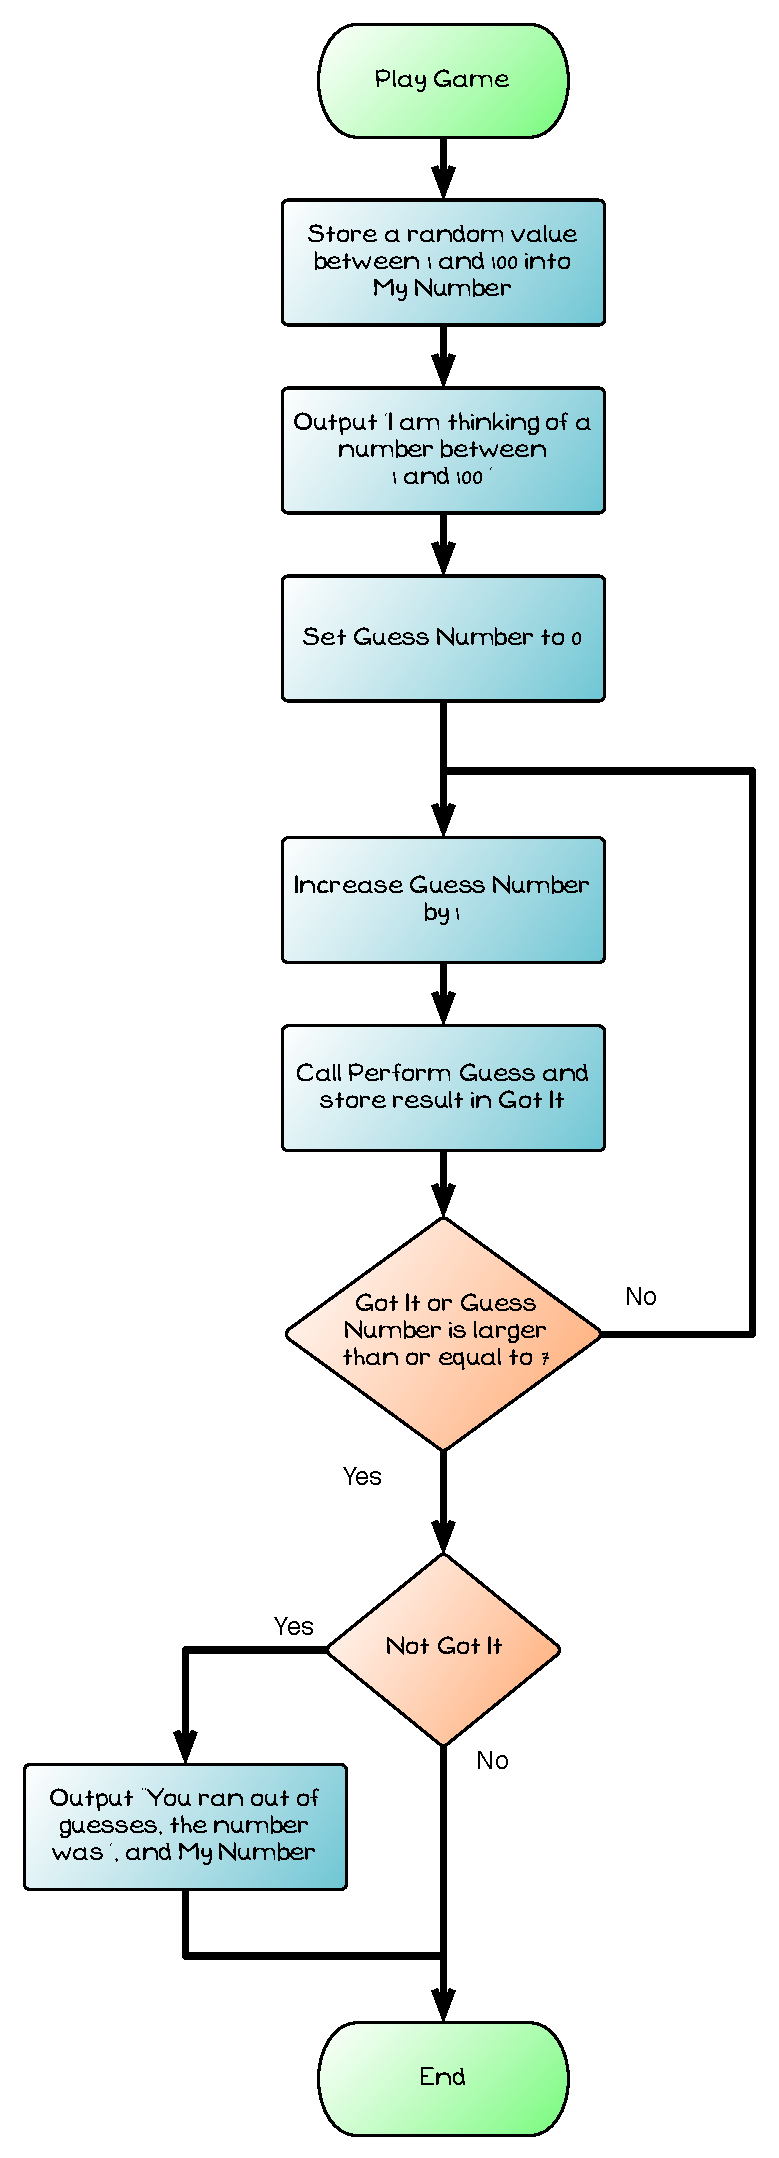
\includegraphics[width=0.52\textwidth]{./topics/control-flow/diagrams/PlayGame} 
   \caption{Logic for the \texttt{Play Game} Procedure}
   \label{fig:play-game}
\end{figure}

\begin{figure}[htbp]
   \centering
   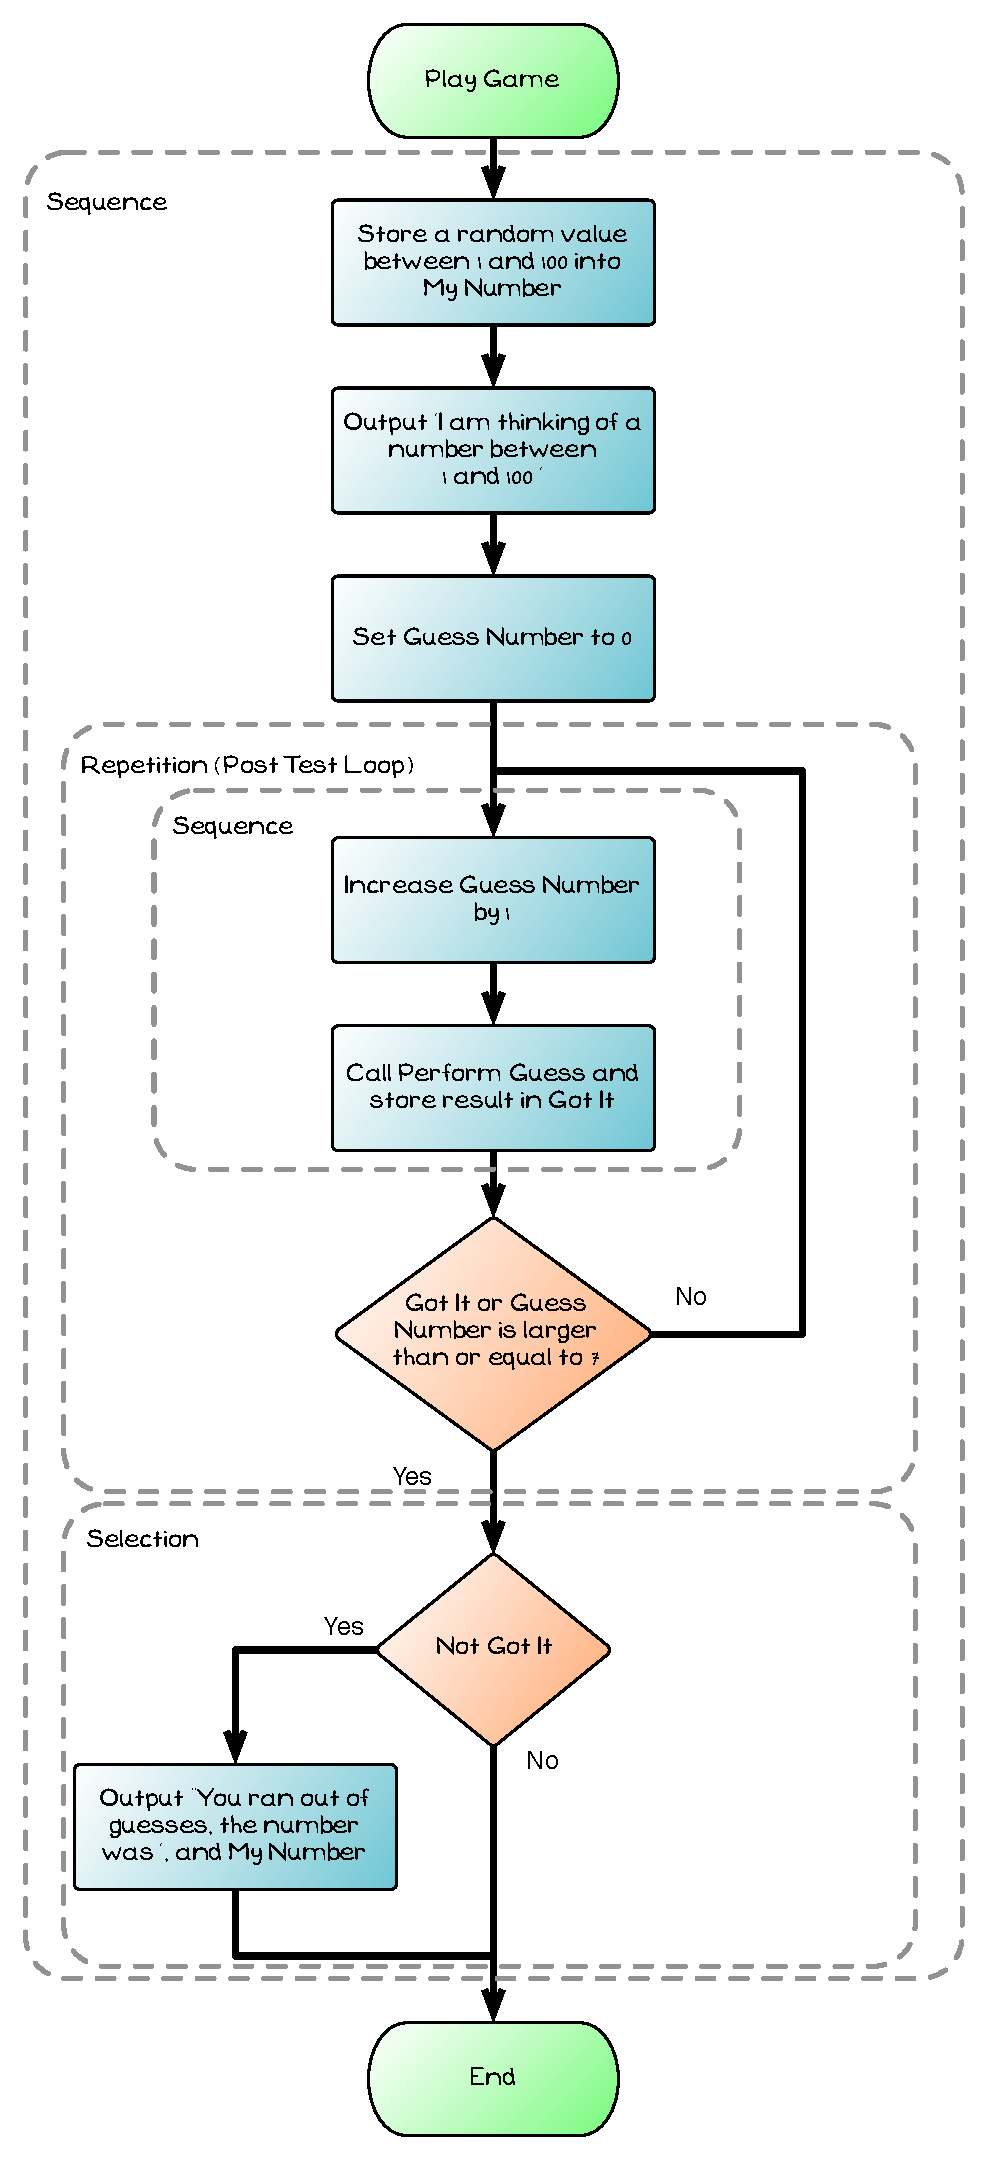
\includegraphics[width=0.65\textwidth]{./topics/control-flow/diagrams/PlayGame1} 
   \caption{Blocks in the \texttt{Play Game} code}
   \label{fig:play-game-diag1}
\end{figure}

\clearpage

\lref{plst:play_game} contains the Pseudocode for the \texttt{Play Game} Procedure. This uses Constants for \texttt{MAX\_NUMBER} and a \texttt{MAX\_GUESSES}, this will make it easier to change the range of the numbers and the associated number of guesses.

The flowchart for \texttt{Play Game} includes a \nameref{sub:post_test_loop}, which can be coded as either a \texttt{do...while} or a \texttt{repeat...until} loop. This two variations are shown in step 7 of \lref{plst:play_game}, with the while version appearing as a comment on the following line. Both of these versions have the same result, but do require different conditions. The two implementations of this are shown in \lref{clst:play_game} and \lref{paslst:play_game}. It is important to understand that the basic ideas of a \textbf{post-test loop} is the same regardless of whether it is coded using \texttt{do...while} or \texttt{repeat...until}.

\pseudocode{plst:play_game}{Pseudocode for \texttt{Play Game}}{topics/control-flow/application/PlayGame.txt}

\mynote{
\begin{itemize}
  \item Notice the indentation make it easier to see which instructions are within the loop and branches of this code.
  \item The C code for this is is \lref{clst:play_game}.
  \item The Pascal code for this is in \lref{paslst:play_game}.
  \item The C and Pascal libraries have different Functions for getting random numbers.
\end{itemize}
}

\csection{In C there is a \texttt{random()} function in the \texttt{stdlib.h} header file. This returns a random integer value. To get this between 1 and MAX\_NUMBER you can use the modulus operator (\%) that returns the remainder after division. The expression to use is \csnipet{random() \% MAX\_NUMBER + 1}}

\passection{In Pascal there is a \texttt{Random} function in the System unit. This takes a single parameter representing the number of random values to generate (0..n-1). The expression to use is \passnipet{Random(MAX\_NUMBER) + 1}}

\clearpage
\csection{\ccode{clst:play_game}{C code for \texttt{Play Game}}{topics/control-flow/application/play-game.c}}

\passection{\pascode{paslst:play_game}{Pascal code for \texttt{Play Game}}{topics/control-flow/application/PlayGame.pas}}

% subsection designing_control_flow_for_play_game (end)

\clearpage
\subsection{Designing Control Flow for Print Line} % (fold)
\label{sub:designing_control_flow_for_print_line}

\texttt{Print Line} is a short Procedure used to print a line of `-' characters to the Terminal. The flowchart for this Procedure is shown in \fref{fig:print-line}, and again with the blocks highlighted in \fref{fig:print-line-diag-1}.

\begin{table}[h]
  \centering
  \begin{tabular}{|c|p{9cm}|}
    \hline
    \multicolumn{2}{|c|}{\textbf{Procedure}} \\
    \hline
    \multicolumn{2}{|c|}{} \\
    \multicolumn{2}{|c|}{\texttt{Print Line}} \\
    \multicolumn{2}{|c|}{} \\
    \hline
    \textbf{Parameter} & \textbf{Description} \\
    \hline
    \texttt{Length} & The number of characters to print. Represents the length of the line. \\
    \hline
    \multicolumn{2}{|c|}{} \\
    \multicolumn{2}{|p{12cm}|}{Prints a number of `-' characters to the Terminal equal. The number of characters to print is specified in the \texttt{Length} parameter.} \\
    \multicolumn{2}{|c|}{} \\
    \hline
  \end{tabular}
  \caption{Specification for the \texttt{Print Line} Procedure.}
  \label{tbl:print line}
\end{table}

\begin{figure}[htbp]
   \centering
   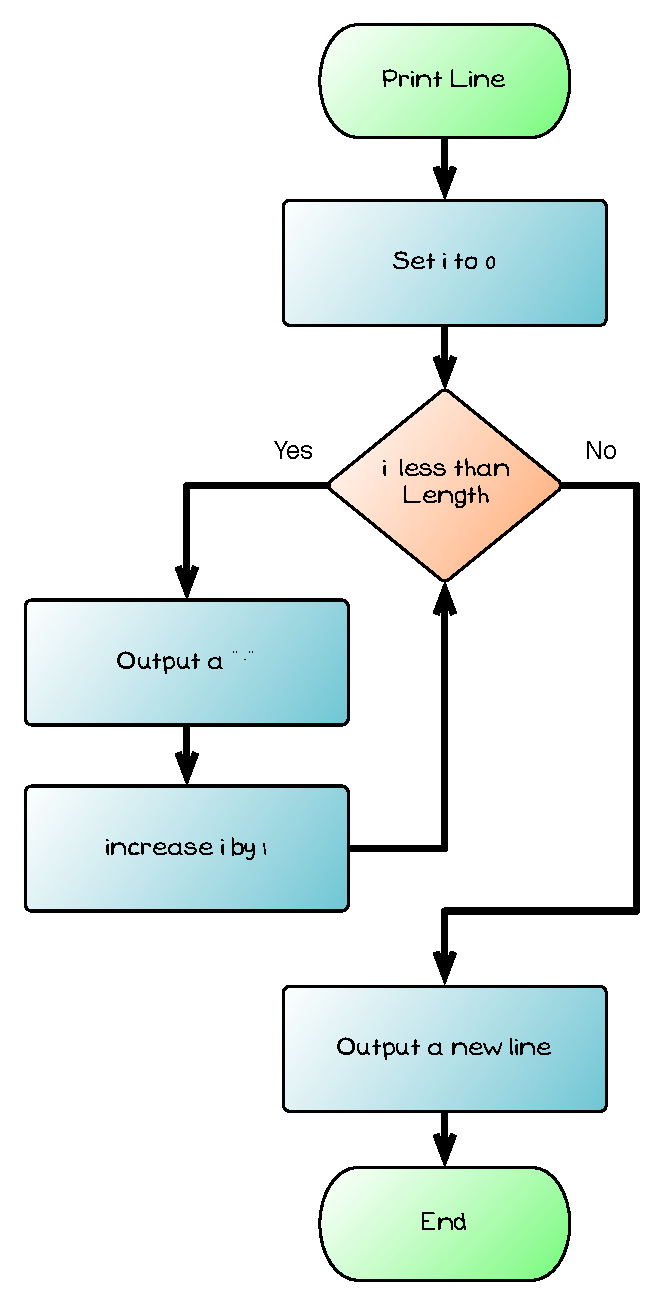
\includegraphics[width=0.37\textwidth]{./topics/control-flow/diagrams/PrintLine} 
   \caption{Flowchart for the logic in \texttt{Print Line} code}
   \label{fig:print-line}
\end{figure}

\clearpage

\begin{figure}[htbp]
   \centering
   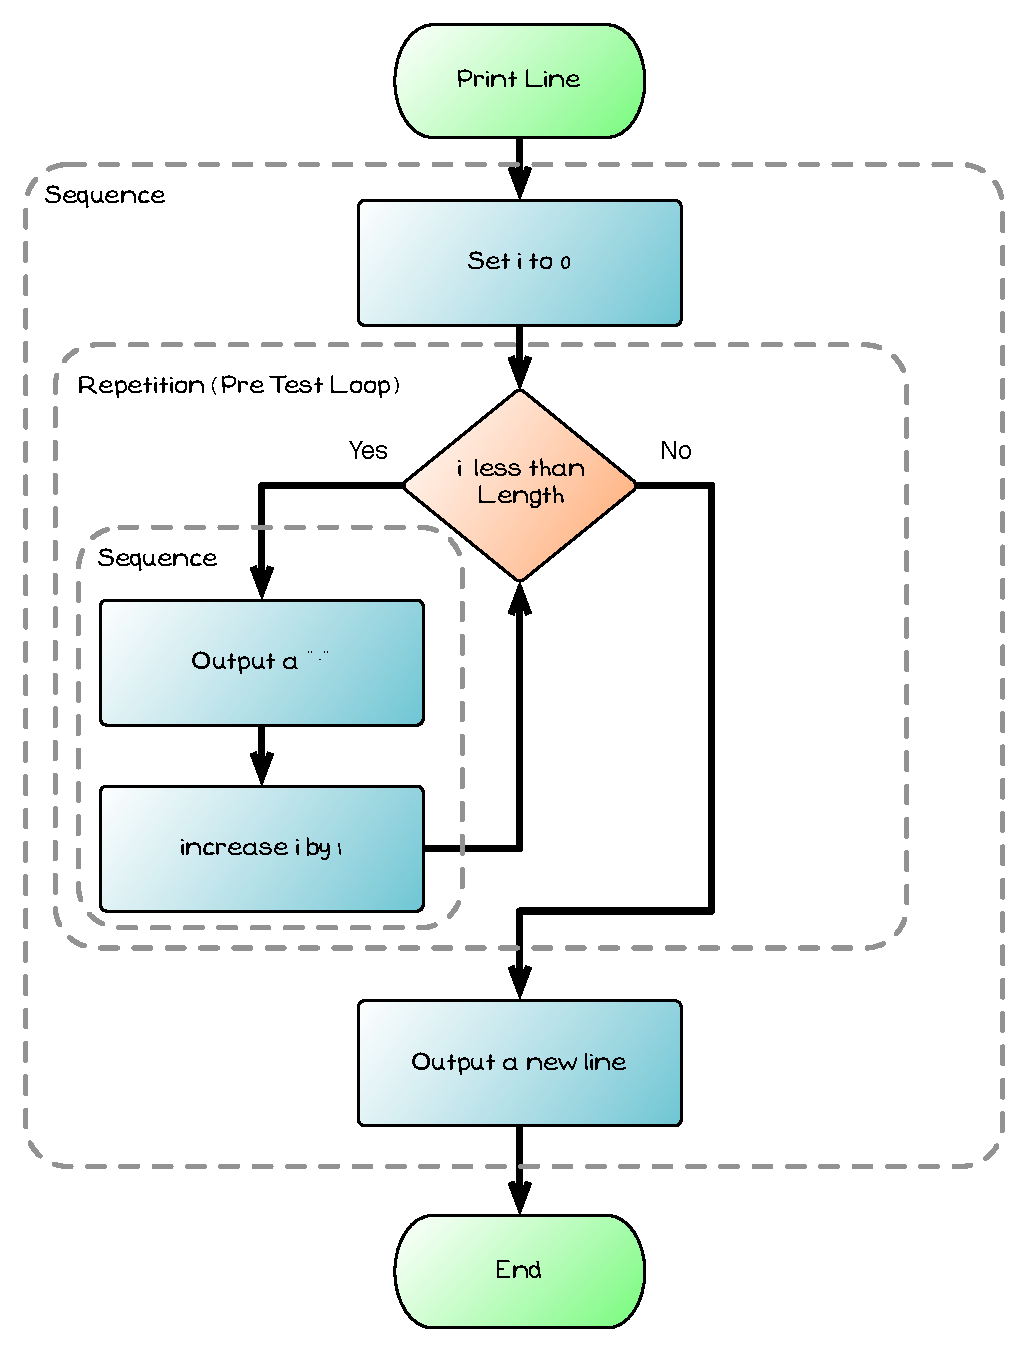
\includegraphics[width=0.57\textwidth]{./topics/control-flow/diagrams/PrintLine1} 
   \caption{Blocks in the \texttt{Print Line} code}
   \label{fig:print-line-diag-1}
\end{figure}

\pseudocode{plst:print_line}{Pseudocode for \texttt{Print Line}}{topics/control-flow/application/PrintLine.txt}

\mynote{
\begin{itemize}
  \item This code includes a \nameref{sub:local_variable} \texttt{i}.
  \item \texttt{i} is used to count the number of times the loop has executed, allowing it to stop when it has printed enough dashes.
  \item This uses a \nameref{sub:pre_test_loop}. This makes sure that no characters are printed if the length is less than or equal to zero.
  \item Notice that a sequence can be placed within a loop.
\end{itemize}
}


% subsection designing_control_flow_for_print_line (end)

\clearpage
\subsection{Designing the Control Flow for Main} % (fold)
\label{sub:designing_the_control_flow_for_main}

The last Procedure is \texttt{Main}. This is responsible for coordinating the actions of the program. It will call \texttt{Play Game} in a loop that repeatedly plays the game until the user decides to quit. \texttt{Main} will have one local variable called \texttt{again}. This will store a character, and will be used to store the value read from the user's response to the `\emph{play again}' prompt.

\begin{figure}[htbp]
   \centering
   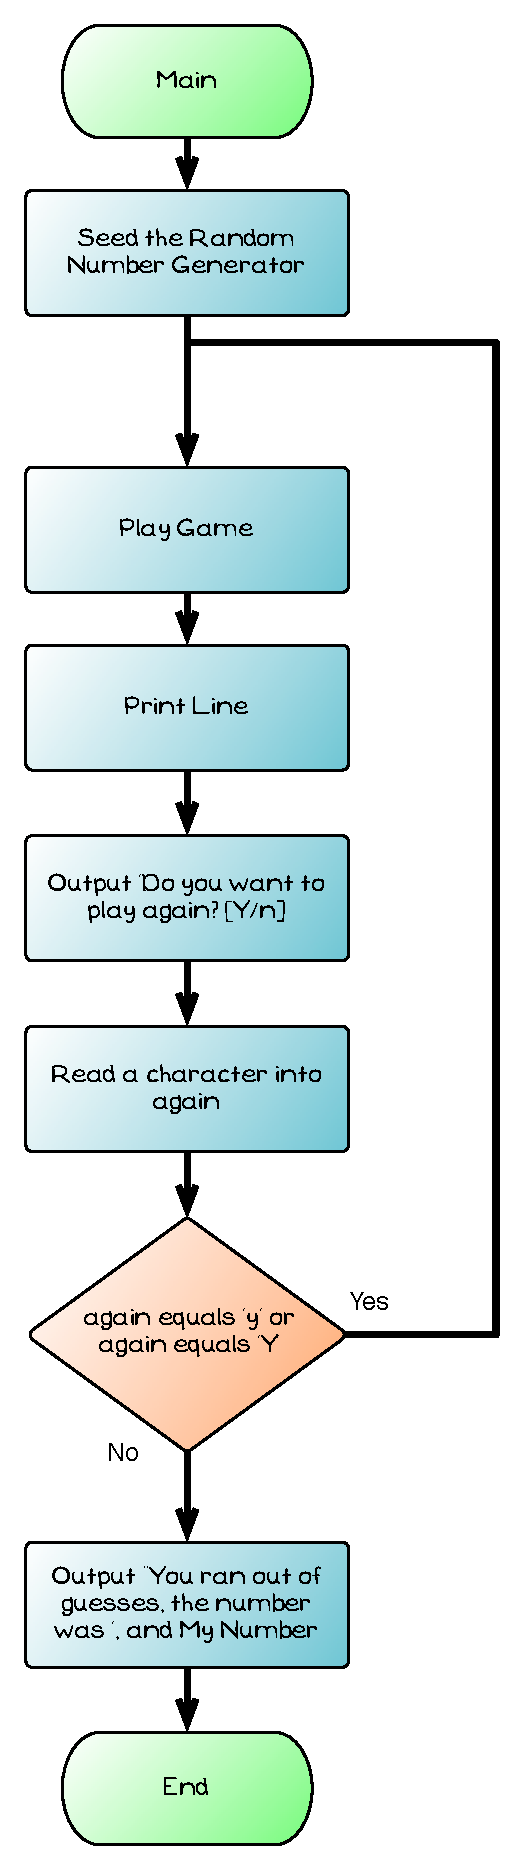
\includegraphics[width=0.31\textwidth]{./topics/control-flow/diagrams/Main} 
   \caption{Flowchart for the \texttt{Main} Procedure}
   \label{fig:main}
\end{figure}

\clearpage

\begin{figure}[htbp]
   \centering
   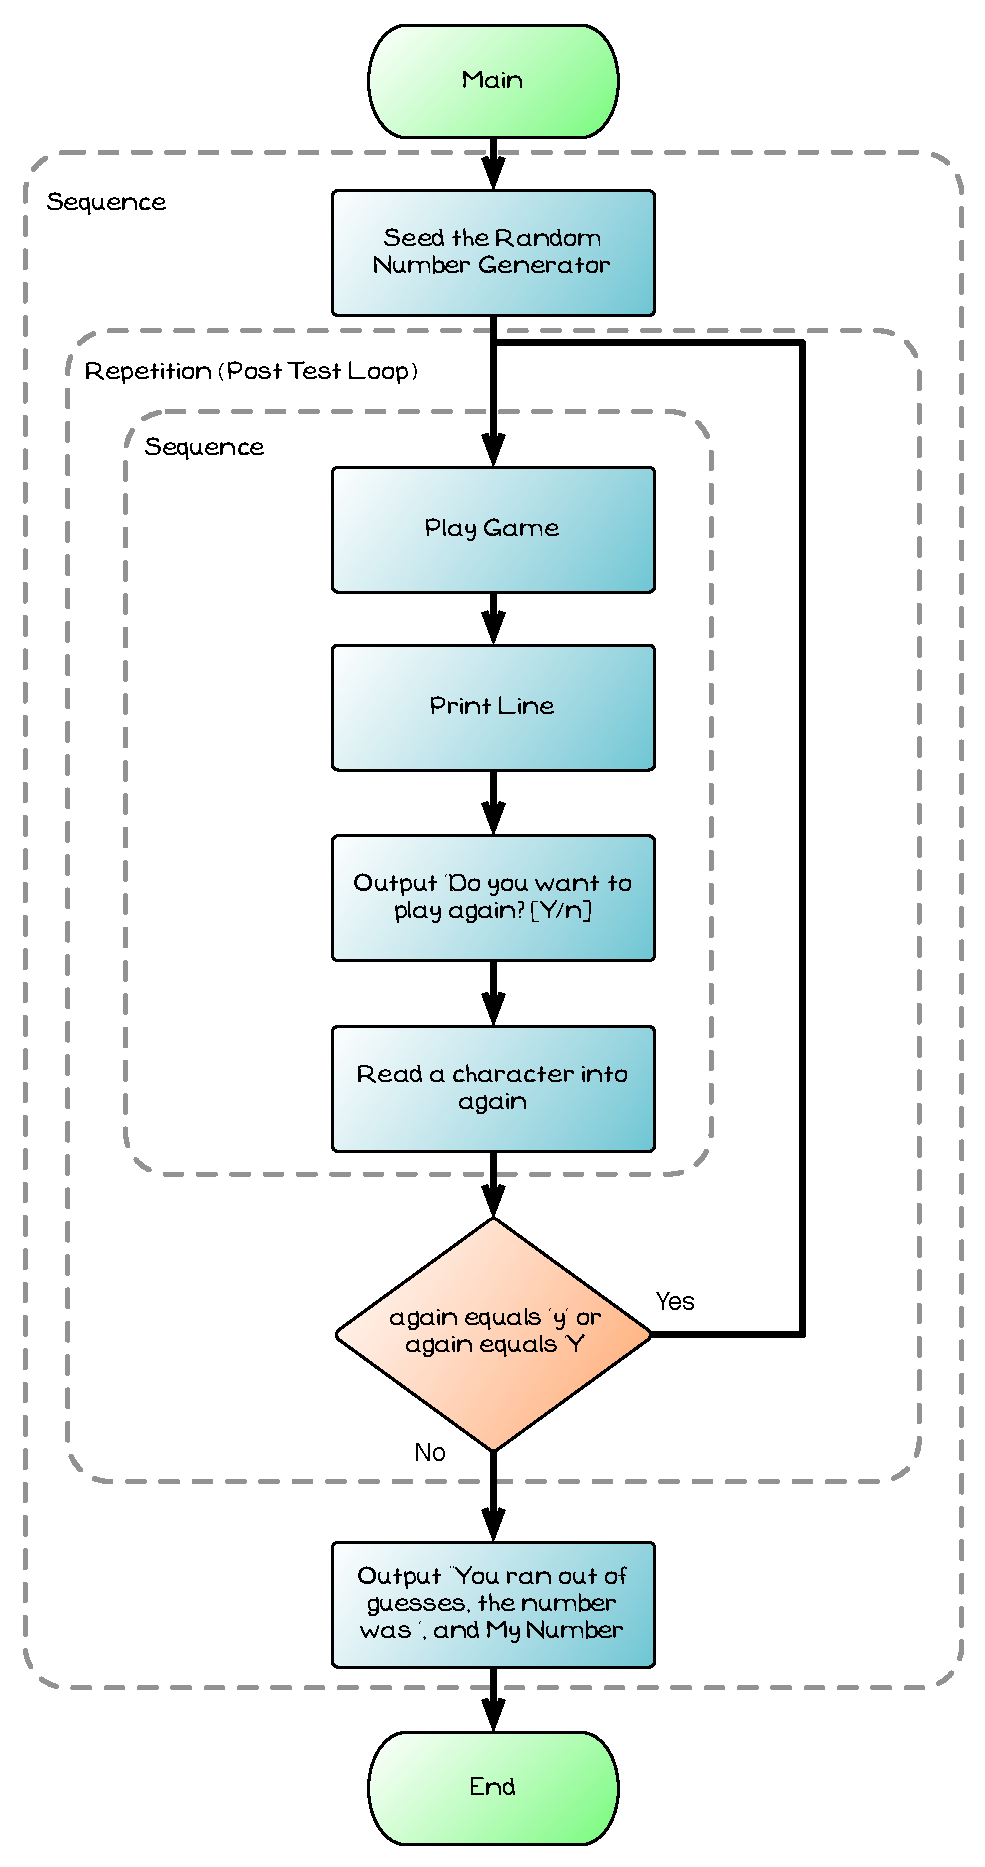
\includegraphics[width=0.55\textwidth]{./topics/control-flow/diagrams/Main1} 
   \caption{Blocks in the \texttt{Main} code}
   \label{fig:main-1}
\end{figure}

\mynote{
Computers cannot generate truly random numbers. Instead it uses a numeric sequence that appears to be random. Seeding the generator with the current time ensures that this random sequence starts at a different value each time the program is run. 
}

% subsection designing_the_control_flow_for_main (end)

\clearpage

\subsection{Writing the Code for Guess That Number} % (fold)
\label{sub:writing_the_code_for_guess_that_number}

Flowcharts and Pseudocode communicate the same ideas. They describe the actions that need to be performed within your code. The following two sections, \sref{sec:control_flow_in_c} \nameref{sec:control_flow_in_c} and  \sref{sec:control_flow_in_pascal} \nameref{sec:control_flow_in_pascal}, contain a description of the syntax needed to code these control flow statements in the C and Pascal programming languages.

\mynote{
Remember the basic process for reading the Syntax Diagrams is to:
\begin{enumerate}
  \item Find the page with the Syntax rule you are interested in knowing about.
  \item Have a quick look at the Syntax Diagram and the rules it contains. Read each rule, and get a basic feel for how it is going to come together for your program.
  \item Read the example to see one way of using the Rule. The Syntax Diagram can be used to create any number of variations of the rule, the example gives you at least one way these rules can be coded.
  \item Return to the diagram and make sure you can match each part of the example back to the rule that created it.
  \item Look up any related rules that are not explained on this rule's page.
\end{enumerate}
}

% subsection writing_the_code_for_guess_that_number (end)

\subsection{Compiling and Running Guess that Number} % (fold)
\label{sub:compiling_and_running_guess_that_number}

Once you have completed the code for this program you need to compile and run it. As this uses random numbers you cannot generate standard test data in order to check the execution. Instead you should perform a number of executions and test the different paths through the program. The main condition you want to check are:
\begin{itemize}
  \item Test failing to get the number in seven guesses.
  \item Test getting the number correct within seven guesses.
  \item Check the output messages when your guess is less than the number (you can enter a guess below 0).
  \item Check the output message when your guess is larger than the number (you can enter a guess larger than 100).
  \item Check that the random sequence is different each time, if its not make sure you have seeded the random number generator.
\end{itemize}



% subsection compiling_and_running_guess_that_number (end)